This chapter first describes a SDN Mininet emulation environment that we use to generate traffic packets (starting from real data patterns) and to retrieve network (feedback) information via the SDN controller, thanks to the OF protocol. Then we shown how to use data collected from such environment to create a predictive model of the switch priority queueing scheuling.

\section{Mininet network emulation environment and control problem} \label{sec:SDNNetSim}
The Mininet environment \cite{Mininet} has been used to emulate a SDN network to validate our methodology in terms of prediction accuracy and control performance. This software runs a collection of virtual network elements (i.e. end-hosts, switches, routers, and links) on a single Linux kernel using lightweight virtualization. 
%To test the effectiveness of the realized controller a simulated network has been programmed using the Mininet environment as a network emulation orchestration system. This software runs a collection of end-hosts, switches, routers, and links on a single Linux kernel by using lightweight virtualization to make a single system look like a complete network. Mininet's virtual objects emulate real SDN network devices. It is usually possible to create a Mininet network that resembles a hardware network, or a hardware network that resembles a Mininet network, and to run the same binary code and applications on either platform.
To generate traffic we used the D-ITG generator \cite{Avallone2004, Botta2012, Botta2013}.

\begin{figure}[tb!]
	\centering
	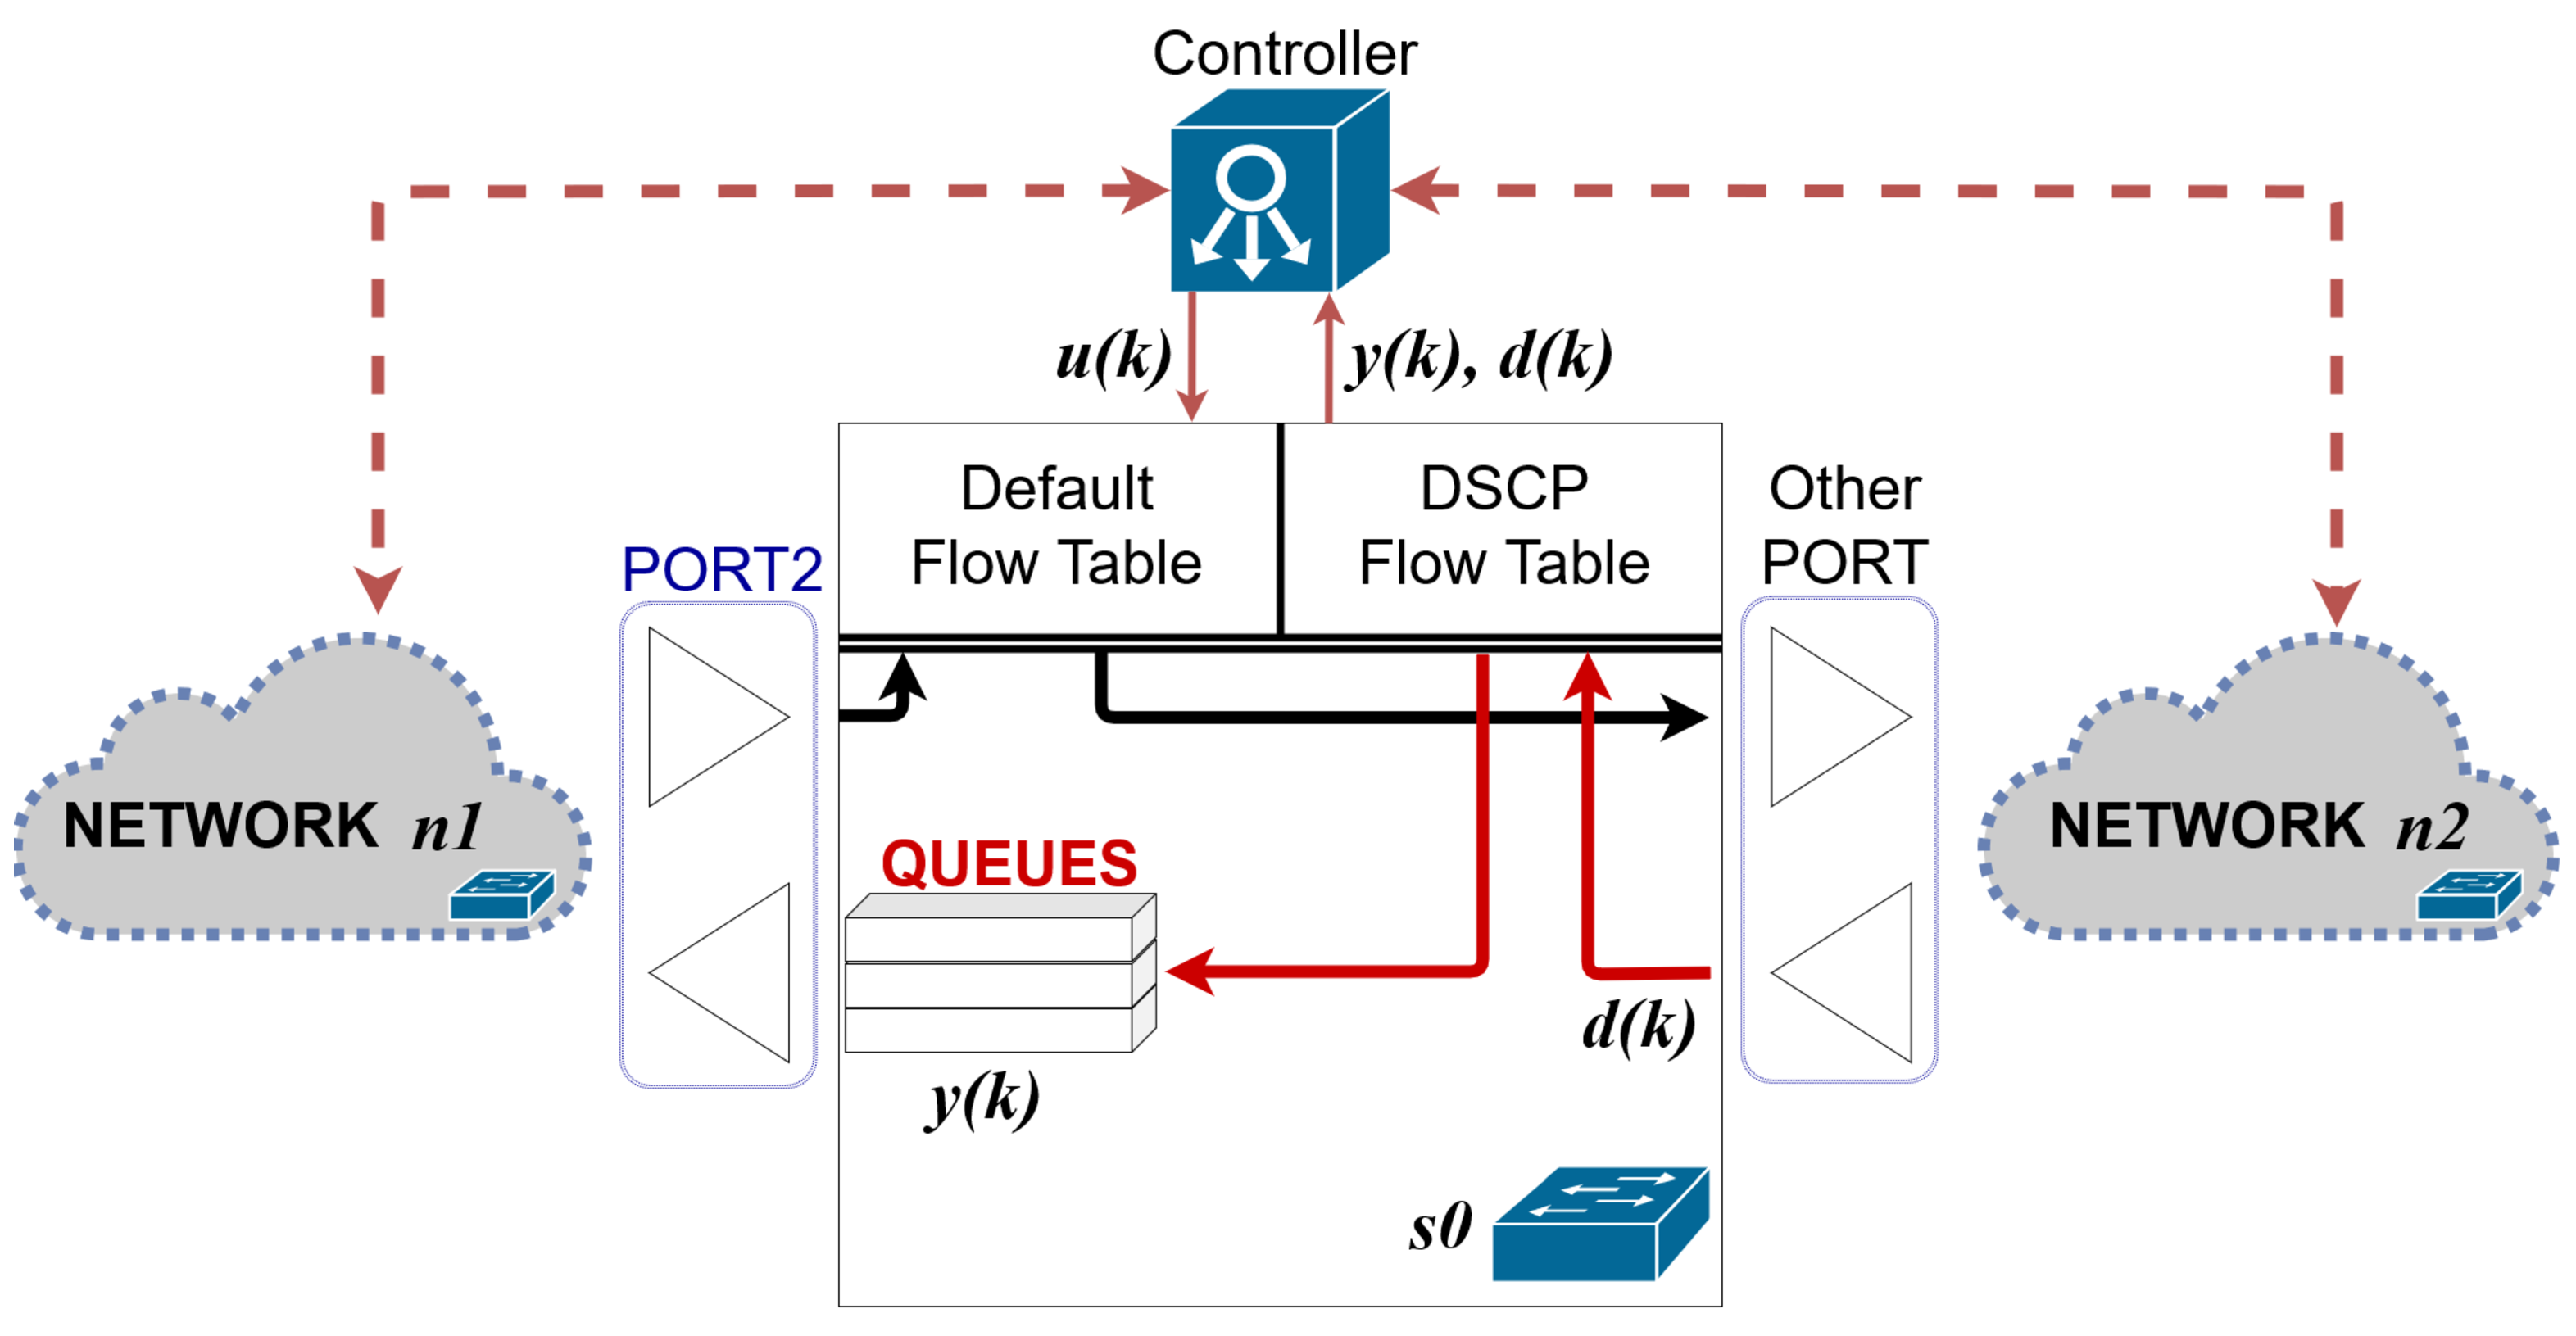
\includegraphics[keepaspectratio,width=\columnwidth]{figure/SDN_net_EPS.eps}
	\caption{Mininet emulated network architecture.}
	\label{fig:{Network}}
\end{figure}
%\begin{figure}[tb!]
%	\centering
%	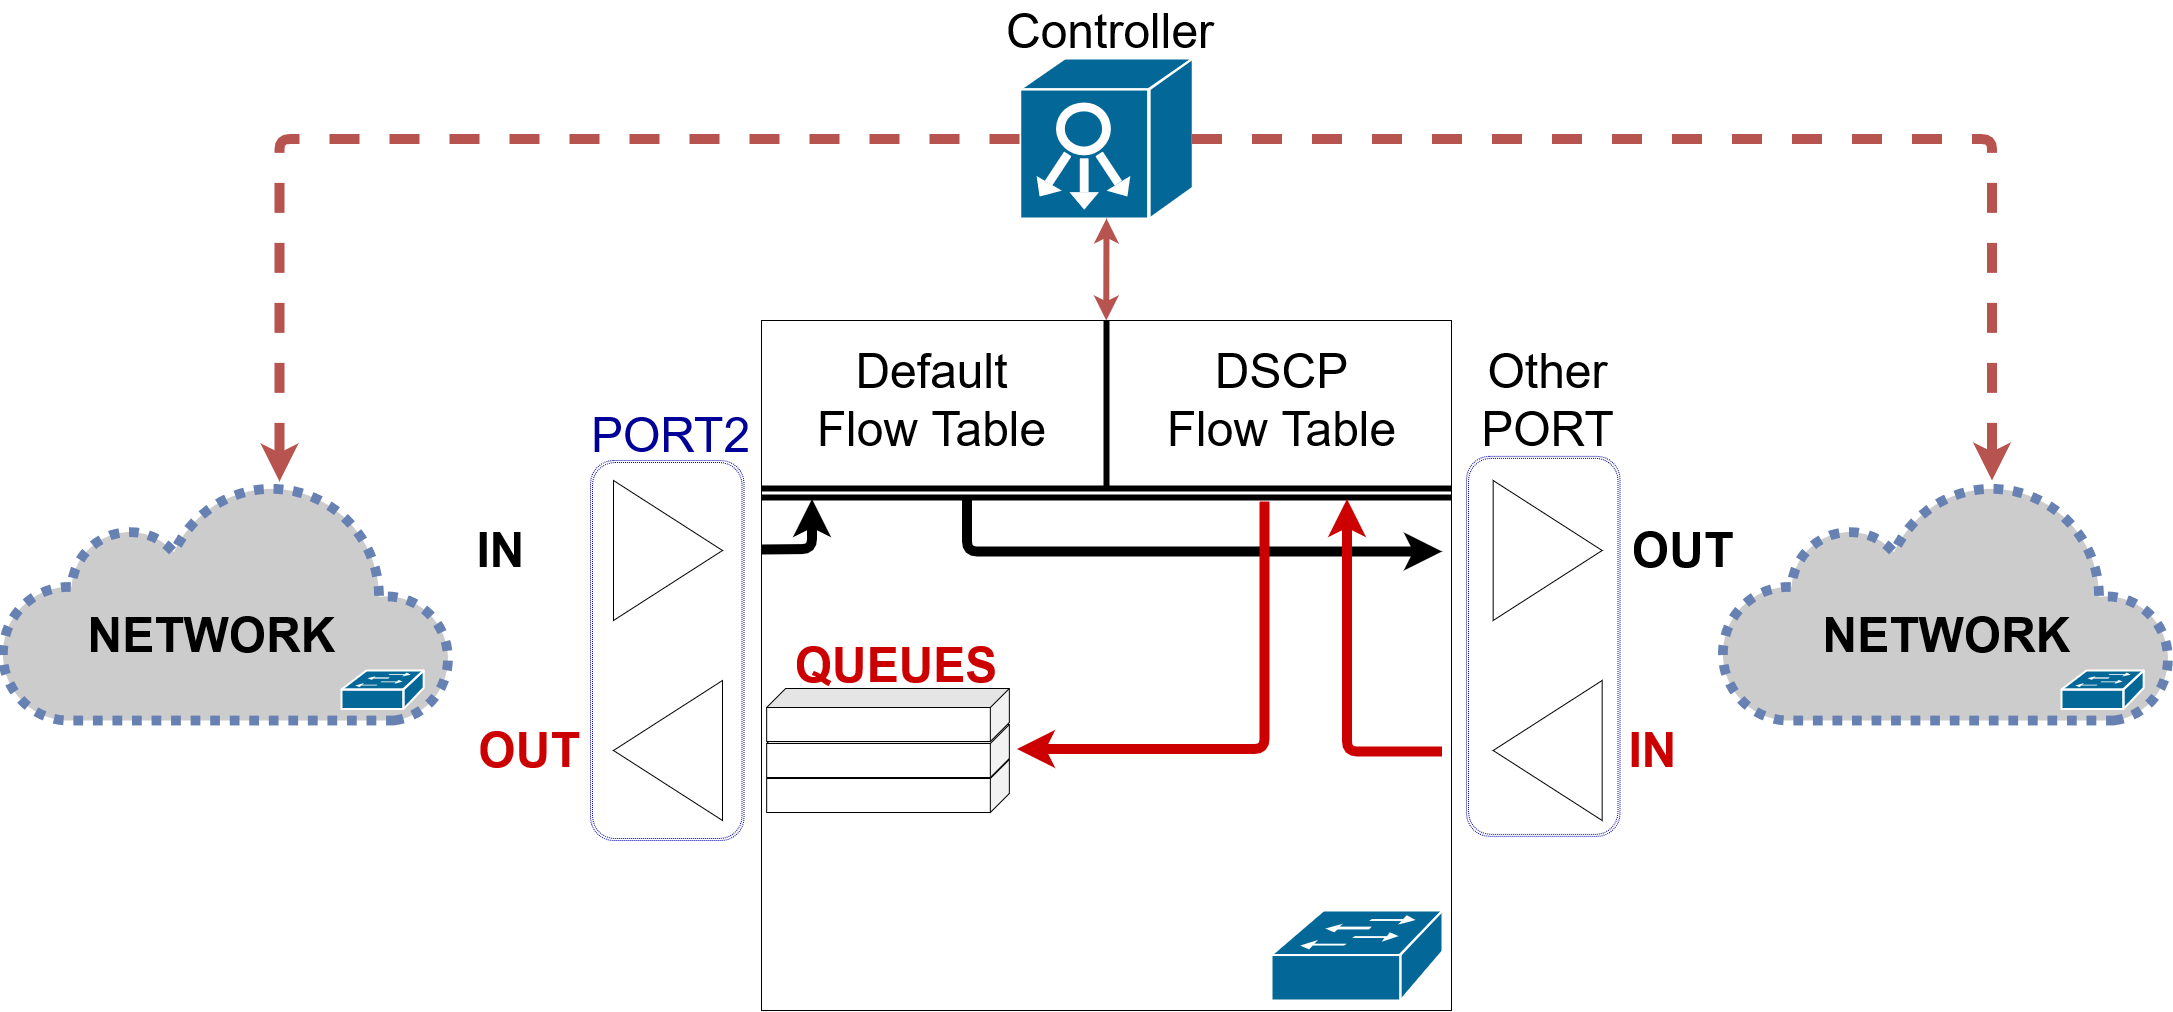
\includegraphics[width=13cm]{figure/SDN_net_LAST.png}
%	\caption{Simulated Network inside Mininet environment.}
%	\label{fig:{Network}}
%\end{figure}

For the purposes of this work, various network configurations were tested. Since similar results has been obtained on all configurations, it is possible to consider the generic case as the architecture in Figure \ref{fig:{Network}}, which aims to represent a portion of a larger network where a bottleneck occurs. More precisely, we consider a switch $s0$ with one input port and one output port, and a remote controller \cite{OVS, RYU} that dynamically manages the configuration of the queues of $s0$. The input of $s0$ is fed with an instance of D-ITG generating stochastic traffic, whose mean value follows the pattern of a real data set (where packets are differentiated by their ToS - Type of Service - priority index) extracted from two days logs of a router of a large service provider network. Namely, the original real data set contains traffic of a real network incoming from a source geographic area and terminating in a destination geographic area, and is divided for each value of Differentiated Services Code Point (DSCP) with a sampling time of 5 minutes \cite{Baker1998, Babiarz2006}. We recall that DSCP is the modern definition of the Type of Service (ToS) field, in which the first 6 bits are the Differentiated Services field that are in common with ToS field, and the last 2 bits regard explicit congestion notification. The ToS field can specify the priority of a datagram and the request for a low delay addressing, a high throughput or a high reliability service. Following the implementation of many national service provider networks (see e.g. \cite{Notiziario}), we partition the 8 different values of the DSCP in three classes: the \textit{Default} class (DSCPs $0,1,3$), the \textit{Premium} (DSCPs $2,4,6,7$), and the \textit{Gold} class (DSCP $5$): to each class we will assign a single queue, associated with a different priority.

%Traffic generation is entrusted to the D-ITG generator which uses informations inside a database created from a real measure that contains the number of packets transmitted and received by a switch. The database fields has been divided for each type of Differentiated Services Code Point (DSCP) with a sampling time of 5 minutes \cite{Baker1998, Babiarz2006}. DSCP is the modern definition of the Type of Service (ToS) field in which the first 6 bits are the Differentiated Services field that are in common with ToS field, and the last 2 bits are the explicit congestion notification. The ToS field can specify the priority of a datagram and the request for a low delay addressing, a high throughput or a high reliability service. Depending on the ToS values, a packet could be placed in a high priority exit queue, or follow a route with latency, throughput and the appropriate reliability for the request.


Using D-ITG Sender and Receiver SW modules it has been possible to establish a connection between networks n1 and n2. In particular, 16 ITG modules have been initialized: 8 for each network, and within each network one for each DSCP index. These modules handle the sampling time interval (5 minutes), the inter-departure time stochastic distribution associated with the packet rate, the packet size stochastic distribution, the IP and port destinations, and the DSCP index. Regarding the controller SW module we used Ryu, which provides software components with well defined Application Programming Interfaces (API) that give the possibility to easily create new network management and control applications. Ryu supports various protocols for managing network devices, such as OpenFlow, Netconf, OF-config, etc. About OF, Ryu supports fully 1.0, 1.2, 1.3, 1.4, 1.5 and Nicira Extensions. For our test-bed the 1.3 version has been chosen. In particular, APIs were used for queue control and counter recovery from the switches \cite{ofctlrest,QoS}. The feedback information collected for the purposes of this work are the descriptions of switches, ports and queues, the number of packets received and transmitted on each port of a switch, the packets passing through the flow tables, the packet rate values of each queue and the packets transmitted by each single queue. In summary, the variables associated to the traffic and control signals in our closed-loop architecture are as follows:

\begin{itemize}
	\item $d(k)\in\Real^{10}$ is a measurable disturbance vector, i.e. representing variables we cannot control. The first 8 components $d_1(k),\ldots,d_8(k)$ consist of the number of packets incoming in the switch $s0$ differentiated with respect to the 8 different values of the DSCPs. $d_9(k)$ and $d_{10}(k)$ are proxy variables, i.e. the hours and minutes of the day, which are very useful to the predictive model since traffic dynamics are tightly correlated with them, e.g. they are substantially different between night and day;
	\item $y(k)\in\Real^{3}$ is the measured output vector, i.e. the variables we want to regulate. They consist of the number of packets outgoing from switch $s0$ differentiated with respect to the corresponding service class: $y_1(k)$ is the Default Queue output, $y_2(k)$ is the Premium Queue output and $y_3(k)$ is the Gold Queue output;
	\item $u(k)\in\Real^{3}$ is the control input vector. Each component corresponds to the queue configuration of each service class: $u_1(k)$ is the Default Queue configuration, i.e. the maximum admitted bandwidth; $u_2(k)$ is the Premium Queue configuration, i.e. the maximum admitted bandwidth; $u_3(k)$ is the Gold Queue configuration, i.e. the minimum admitted bandwidth;
\end{itemize}

\begin{figure}[tb!]
	\centering
	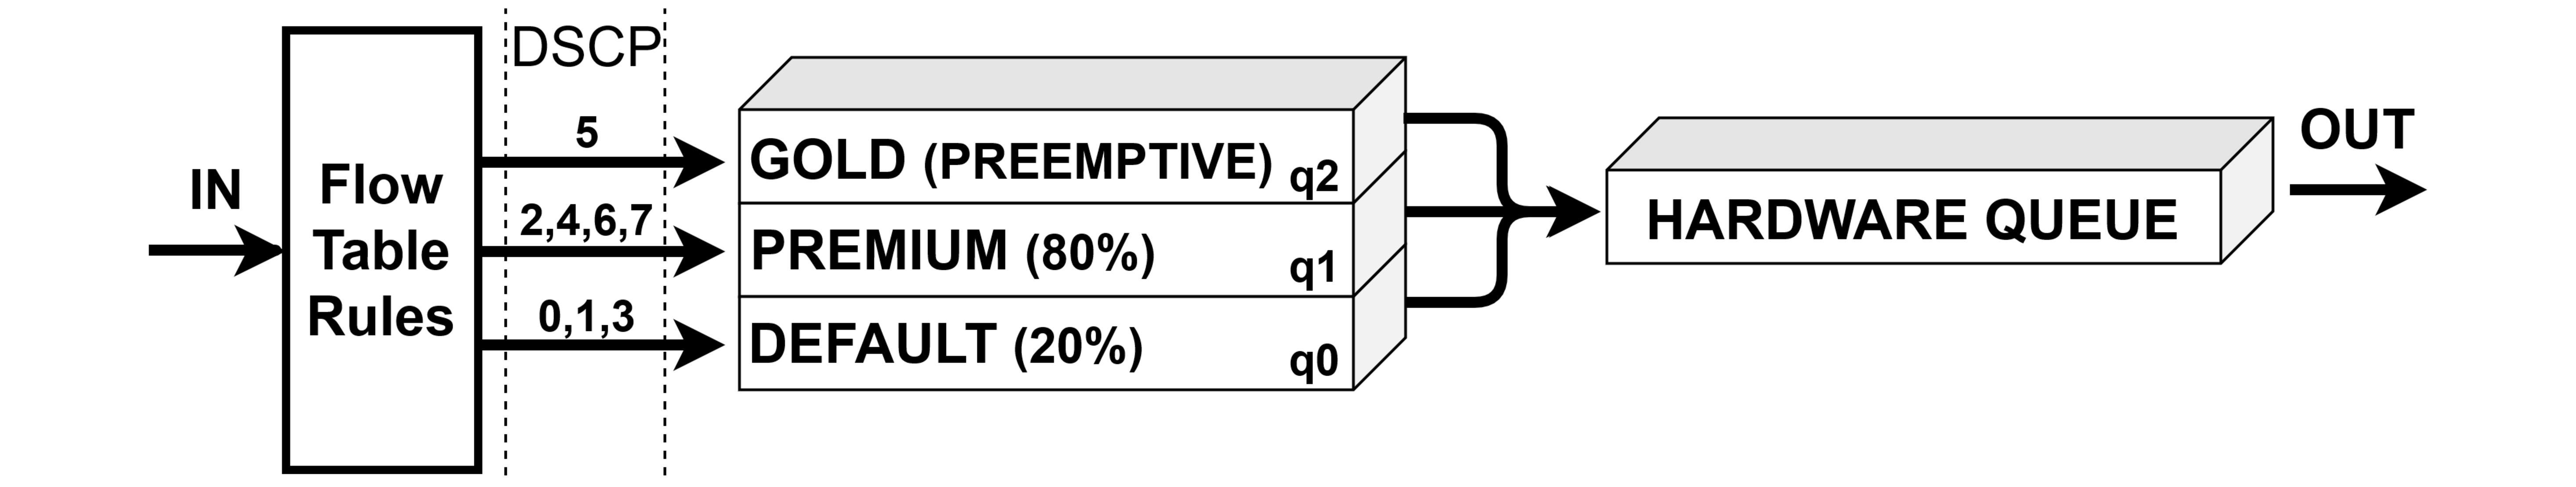
\includegraphics[keepaspectratio,width=\columnwidth]{figure/QUEUE.eps}
%	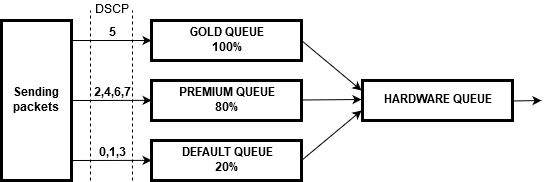
\includegraphics[keepaspectratio,width=12cm]{figure/queue.png}
	\caption{Static queues rate with routed packets relative to DSCP.}
	\label{fig:{queue}}
\end{figure}

In this work we first applied in our emulative scenario the static control of queues used in the Italian service provider network of \textit{Telecom Italia} \cite{Notiziario}, which is depicted in Figure \ref{fig:{queue}}. To this aim we defined 3 queues in $s0$ and configured the queues as follows: packets with the DSCP values 0, 1 and 3 (Default queue) are routed via queue 0, with maximum rate $u_1(k) = 20 \textit{MB/s}, \forall k$; the packets with values 2, 4, 6 and 7 (Premium queue) are routed on queue 1, with maximum rate $u_2(k) = 80 \textit{MB/s}, \forall k$; the packets with value 5 (Gold queue) are routed on queue 2, with minimum rate $u_3(k) = 100 \textit{MB/s}, \forall k$. To obtain this prioritization it has also been necessary to set the flow tables of $s0$ to discriminate incoming packets based on the DSCP value and the destination IP address, and re-route them to the desired queue. Also, to obtain a bottleneck situation in $s0$, we have chosen the bandwidth of the output port of switch $s0$ at 100 \textit{MB/s}. Using this configuration queue 2 uses the maximum capacity of the port to forward packets with preemptive priority, while the other two queues use the remaining bandwidth from 0 \textit{MB/s} to the specified maximum bandwidth based on needs.
%As formally defined later in Section \ref{secSwitchedModeling}, the packets sent by the queues will be collected in the state vector to be controlled $x(k)\in\mathbf{R}^3,\ \forall k$,  while the bandwidth associated to the queues will compose the control variables vector $u(k)\in\mathbf{R}^3,\ \forall k$.
To instantiate the chosen topology in Mininet it has been necessary to run the \ref{Topology} code from the Ubuntu command line with the following text:
\Blackline{ sudo python Topology\textunderscore qos.py}
\noindent In this script all network devices (remote controller, switches and hosts), their attributes and their connections are defined. Furthermore this script is also responsible for the traffic generated between hosts thanks to the function defined within the \ref{ditg} code that is iteratively used every five minutes to read the provided real data traffic database and generate the synthetic traffic inside the network. In lines $49$ to $53$ of \ref{Topology} code Mininet adds an external controller, Ryu in our case, to specified IP address and port. Obviously it is necessary that the controller is already instantiated before launching the network topology, and it is possible to do this through the following command:
\Blackline{ ryu run main\textunderscore controller\textunderscore TOS.py rest\textunderscore qos.py rest\textunderscore conf\textunderscore switch.py ofctl\textunderscore rest.py}
\noindent This command executes several scripts, the first one (\ref{main_controller_TOS}) is the Ryu controller which invokes additional functions designed for saving network information and setting queue bandwidths (from \ref{datapath_monitor_TOS} to \ref{qos_simple_switch_13}). The remaining scripts are all the rest APIs required for these features to work properly (\ref{ofctl_rest}, \ref{rest_conf_switch} and \ref{rest_qos} codes).

As we will see in Section \ref{secExpRes}, using static priority control the queues will not be able to send all the packets incoming from network $n1$, and a dramatic amount of packets will be lost. This motivates the application of optimization techniques, which are enabled by the predictive models derived using the methodology described in section \ref{secSwitchedModeling}.

\section{Regression Trees and Random Forest based models for MPC}\label{secSwitchedModeling}
In this section a methodology to apply the results proposed in \cite{SmarraADHS2018,smarraNAHS2020} is illustrated, to identify, starting from a set of collected historical data $ \mathcal{D}=\{y(k),u(k),d(k)\}_{k = 0}^{\ell} $ (generated as described in the previous section), a switching ARX model of the input-output behavior of the traffic flow in a switch of a SDN network as follows:
%The aim of such predictive model is to enable the direct and computationally efficient implementation of Model Predictive Control for bandwidth and packet losses optimisation.
%\small
\begin{equation}\label{eqIdentifiedModelNSARX}
x(k+j+1) =	A'_{\sigma_j(x(k),d(k))} x(k) + \sum_{\alpha = 0}^{j}B'_{\sigma_{j}(x(k),d(k)),\alpha} u(k+\alpha) + f'_{\sigma_j(x(k),d(k))},
\end{equation}
%\normalsize
\noindent $j = 0,\ldots, N-1$, where $x(k) \doteq [y^\top(k)\ \cdots\ y^\top(k-\delta_y)\ u^\top(k-1)\ \cdots\ u^\top(k-\delta_u)]^\top\in\Real^{n_x}$ is an extended state to characterize a switching ARX model, with $x_\iota(k) \doteq [y_\iota(k)\ \cdots\ y_\iota(k-\delta_y)\ u^\top(k-1)\ \cdots\ u^\top(k-\delta_u)]^\top\in\Real^{\delta_y+1+3\delta_u}$, $\iota = 1,2,3$, $N$ is the chosen future predictive horizon, and  $\sigma_j : \mathbb{R}^{n_x+10} \to \mathcal M \subset \mathbb{N}$ is a switching signal that associates an operating mode in a finite set $\mathcal M$ to each pair $(x(k),d(k))$ and each prediction step $j$ of the horizon.
It is possible to directly use model \eqref{eqIdentifiedModelNSARX} to setup the following problem, which can be solved using standard Quadratic Programming (QP) solvers:\\
\begin{problem}\label{pbMPCSwitching}
%	\small
	\vspace{-0.3cm}
	\begin{equation*}
		\begin{aligned}
			& \underset{u_0,\ldots,u_{N-1}}{\text{minimize}} & &  \sum_{j=0}^{N-1} \left(\left(x_{j+1}-x_{\mathrm{ref}}\right)^\top Q \left(x_{j+1}-x_{\mathrm{ref}}\right) + u^\top_{j} R u_{j}\right)\\
			& \text{subject to }            & &  x_{j+1} = A'_{\sigma_j(x_{0},d_{0})} x_0 + \sum_{\alpha = 0}^{j}B'_{\sigma_{j}(x_{0},d_{0}),\alpha} u_\alpha + f'_{\sigma_j(x_{0},d_{0})}\\       
			&                               & &  u_{j}   \in \mathcal{U}\\
			&                               & &  x_{0} = x(k), d_{0} = d(k)\\ 
			&                               & &  j = 0,\ldots,N-1.			\\
		\end{aligned}
		\vspace{0.1cm}
	\end{equation*}
%	\normalsize
\end{problem}
\noindent As it is well known \cite{borrelli2017predictive}, Problem \ref{pbMPCSwitching} is solved at each time step $k$ using QP to compute the optimal sequence $u^*_0,\ldots,u^*_{N-1}$, but only the first input is applied to the system, i.e. $u(k) = u^*_0$. Note that, for any prediction step $j$, $x_{j+1}$ only depends on the measurements $x_0=x(k),d_0=d(k)$ at time $k$, since they are the only available measurements at time-step $k$. 
%\subsection{Switching ARX Identification using RF}\label{secSARX}

\subsection{RT and RF background}
Let us consider a dataset $\{y(k),x_1(k),\ldots,x_\eta(k)\}_{k=0}^\ell$, with $y,x_1,\ldots,x_\eta\in\mathbb{R}$. Let us suppose  to estimate, using Regression Trees, the prediction of the (response) variable $y(k)$ using the values of predictor variables $x_1(k),\ldots,x_\eta(k)$. The CART algorithm \cite{BreimanCART2017} creates a RT structure via optimal partition of the dataset. It solves a Least Square problem by optimally choosing recursively a variable to split and a corresponding splitting point. After several steps the algorithm converges to the optimal solution, and the dataset is partitioned in hyper-rectangular regions (the leaves of the tree) $R_1, R_2,\cdots, R_\nu$. In each partition $y(k)$ is estimated with a different constant $\hat y_i\, i=1,\ldots,\nu,$ given by the average of the samples of $y(k)$ falling in $R_i$, i.e.

\begin{equation}\label{eqAverageResponseRT}
\hat y_{i} = \frac{\sum\limits_{\{k|(x_1(k),\ldots, x_\eta(k)) \in R_i\}}y(k)}{|R_i|}
\end{equation}


\noindent Random Forests \cite{BreimanML2001} are instead an averaging method that exploits a combination of tree predictors such that each tree depends on the values of a random vector sampled independently and with the same distribution for all trees in the forest. The output prediction is given by averaging the predictions provided by all trees in the forest. It is possible to show that the error introduced by the forests quickly and almost surely converges to a limit as the number of trees in the forest becomes large. Such error also depends on the strength of the individual trees in the forest and the correlation between them. Thus, due to the Law of Large Numbers, Random Forests (differently from Regression Trees) do not suffer much variance and overfitting problems. For more details the reader is refered to \cite{BreimanCART2017,BreimanML2001}.

\subsection{Switching ARX (SARX) model identification via RT} To derive a model as in \eqref{eqIdentifiedModelNSARX}, a new dataset $\X= \{x(k),u(k),d(k)\}_{k = 0}^{\ell}$ has to be defined starting from $\D$. In order to apply MPC it is needed, for each component of $y(k)$, a model that can predict system's dynamics over a horizon of length $N$. The idea is to create $3 N$ predictive trees $\{\mathcal{T}_{\iota,j}\},\ \iota=1,2,3,\ j=0,\ldots,N-1$, each one to predict the 3 outputs components of the system over the $N$ steps of the horizon. To create the tree structure, the RT algorithm (CART) partitions the dataset $\X$ into regions $\X_i$, such that $\biguplus \X_i = \X$, and assigns to each region a constant value given by the average of the output values of the samples that ended up in that leaf. In run-time, once the trees are created, and given a real-time measurement $(x(k), u(k), d(k))$ belonging to leaf $i$, the CART algorithm provides as a prediction the averaged value associated to the leaf as in \eqref{eqAverageResponseRT}. However, since the prediction provided by the RT is a constant value, it cannot be used to setup an MPC problem, thus the learning procedure needs to be modified to identify a modeling framework as in \eqref{eqIdentifiedModelN}. To this end, $\X$ is partitioned in two disjoint sets $\mathcal{X}_c = \{u(k)\}_{k=0}^{\ell}$ of data associated to the control variables, and $\mathcal{X}_{nc} = \{(x(k), d(k))\}_{k=0}^{\ell}$ of data associated to remaining variables, and then apply the CART algorithm only on $\mathcal{X}_{nc}$ (this is to avoid that the MPC problem turns out into a Mixed Integer Quadratic Program, see \cite{SmarraADHS2018,smarraNAHS2020} for details); thus, $3 N$ RTs $\{\mathcal{T}_{\iota,j}\}$ have been created, each constructed to predict the variable $y_\iota(k+j+1)$, and consequently $x_\iota(k+j+1)$. In particular, it is associated to each leaf $\iota,i_j$, corresponding to the partition  $\mathcal{X}_{nc,\iota,i_j}$, of each tree $\mathcal{T}_{\iota,j}$ the following affine model is associated

%\small
%
\begin{equation}\label{eqLTIleavesSinglState}
	x_\iota(k+j+1) = A'_{\iota,i_j}x(k) + \sum_{\alpha = 0}^{j}{B'_{\iota,i_j,\alpha}u(k+\alpha)} + f'_{\iota,i_j},
\end{equation}
%\normalsize
%\small
\begin{equation}\label{eqLeafModel}
\begin{aligned}
A'_{\iota,i_j} =& \left[\begin{array}{cccccccccc}
a_1       & a_2       & \cdots & a_{\delta_y } & a_{\delta_y + 1} & b_{\delta_y + 2} & \cdots & b_{\delta_y + 1+ 3(\delta_u-1)} & \cdots & b_{\delta_y + 1 + 3\delta_u} \\
1         & 0         & \cdots & 0             & 0                & 0                & \cdots & 0                               & \cdots & 0                            \\
\vdots    & \vdots    & \ddots & \vdots        & \vdots           & 0                & \cdots & 0                               & \cdots & 0                            \\
0         & 0         & \cdots & 1             & 0                & 0                & \cdots & 0                               & \cdots & 0                            \\
0         & 0         & \cdots & 0             & 0                & 0                & \cdots & 0                               & \cdots & 0                            \\
0         & 0         & \cdots & 0             & 0                & 0                & \cdots & 0                               & \cdots & 0                            \\
0         & 0         & \cdots & 0             & 0                & 0                & \cdots & 0                               & \cdots & 0                            \\
0         & 0         & \cdots & 0             & 0                & 1                & \cdots & 0                               & \cdots & 0                            \\
\vdots    & \vdots    & \ddots & \vdots        & \vdots           & \vdots           & \ddots & \vdots                          & \ddots & \vdots                       \\
0         & 0         & \cdots & 0             & 0                & 0                & \cdots & 1                               & \cdots & 0                            \\

\end{array}\right],\\
B'_{\iota,i_j,\alpha} = & \left[\begin{array}{ccc}
b_{1,\alpha} & b_{2,\alpha} & b_{3,\alpha}\\
0            & 0            & 0            \\
\vdots       & \vdots       & \vdots \\
0            & 0            & 0            \\   
0            & 0            & 0            \\  
0            & 0            & 0            \\  
0            & 0            & 0            \\  
0            & 0            & 0            \\  
\vdots       & \vdots       & \vdots            \\   
0            & 0            & 0            \\   
\end{array}\right],\ \alpha<j,\ 
B'_{\iota,i_j,j} =  \left[\begin{array}{ccc}
b_{1,\alpha} & b_{2,\alpha} & b_{3,\alpha}\\
0            & 0            & 0            \\
\vdots       & \vdots       & \vdots \\
0            & 0            & 0            \\   
1            & 0            & 0            \\  
0            & 1            & 0            \\  
0            & 0            & 1            \\  
0            & 0            & 0            \\  
\vdots       & \vdots       & \vdots            \\   
0            & 0            & 0            \\   
\end{array}\right],\ 
f'_{\iota,i_j} = \left[\begin{array}{ccccc}
f      \\	0 \\ \vdots \\ 0 \\ 0 \\ 0 \\ 0 \\ 0 \\ \vdots \\ 0      
\end{array}\right],
\end{aligned}
\end{equation}
%\normalsize

\noindent where the coefficients of matrices $A'_{\iota,i_j}$, $B'_{\iota,i_j,\alpha}$ and $f'_{\iota,i_j}$ are obtained in each leaf $\iota,i_j$ by fitting the corresponding set of samples solving the following Least Squares with inequality constraints problem:

\begin{problem}\label{pbLeastSquareProblem}
%	\small
	\begin{alignat}{2}
		& \nonumber \underset{\xi_{\iota,i_j}}{\text{minimize}} & &  \parallel \Lambda_{\iota,i_j} \xi_{\iota,i_j}  - \lambda_{\iota,i_j} \parallel_2^2   		 \\
		& \text{subject to }    \nonumber            & &  f_\mathrm{min} \leq f \leq f_\mathrm{max}    										  					 \\
		&                  					    	 & &  a_\mathrm{min} \leq a_{\jmath} \leq a_\mathrm{max}\label{eqInequalityConstraints} \\
		& 	                    \nonumber			 & &  b_\mathrm{min} \leq b_{\iota,\alpha} \leq b_\mathrm{max},
	\end{alignat}
%	\normalsize
\end{problem}

\noindent where $\xi_{\iota,i_j}$, $\lambda_{\iota,i_j}$, and $\Lambda_{\iota,i_j}$ contain respectively the parameters of matrices in \eqref{eqLeafModel}, the predictions $x_\iota(k+j+1)$, and the current measurements of $x(k)$ and $u(k+\alpha)$. Linear inequalities \eqref{eqInequalityConstraints} are used to constrain elements in $\xi_{\iota,i_j}$ to take into account physical system constraints and improve prediction accuracy.
Model \eqref{eqLTIleavesSinglState} can be easily compacted in the following form taking into account all the states $\iota=1,2,3$:
%\small
\begin{equation}\label{eqLTIleavesCompact}
x(k+j+1) = A'_{i_j}x(k) + \sum_{\alpha = 0}^{j}{B'_{i_j,\alpha}u(k+\alpha)} + f'_{i_j}.
\end{equation}
%\normalsize
\noindent In particular, with the specific choice of $\delta_u = 0$ model \eqref{eqIdentifiedModelNSARX} can be rewritten in the following state-space formulation
%\small
\begin{equation}\label{eqIdentifiedModelN}
x(k+j+1) =	A_{\sigma_j(x(k),\bold{u^-}(k),d(k))} x(k+j) + B_{\sigma_j(x(k),\bold{u^-}(k),d(k))} u(k+j) + f_{\sigma_j(x(k),\bold{u^-}(k),d(k))},
\end{equation}
%\normalsize
where $\bold{u^-}(k) = [u^\top(k-1)\ \cdots\ u^\top(k-\delta)]^\top$ is the vector with the regressive terms of the input used to only grow the trees, and  $\sigma_j : \mathbb{R}^{3(\delta_y+1)+3\delta+10} \to \mathcal M \subset \mathbb{N}$.
%\noindent In particular, as anticipated in the problem formulation, with the specific choice of $\delta_u = 0$ matrices $A'_{\iota,i_j}$ in \eqref{eqLeafModel} modify as follows:
%
%\small
%\begin{equation}\label{eqLeafModelDelta_u=0}
%	\begin{aligned}
%		A'_{\iota,i_j} =& \left[\begin{array}{ccccc}
%			a_1       & a_2       & \cdots & a_{\delta_y } & a_{\delta_y + 1} \\
%			1         & 0         & \cdots & 0                         & 0     \\
%			\vdots    & \vdots    & \ddots & \vdots                    & \vdots     \\
%			0         & 0         & \cdots & 1                         & 0     
%		\end{array}\right]\\
%		B'_{\iota,i_j,\alpha} = & \left[\begin{array}{ccccc}
%			b_{1,\alpha} & 0 & \cdots & 0 & 0\\
%			b_{2,\alpha} & 0 & \cdots & 0 & 0           \\
%			b_{3,\alpha} & 0 & \cdots & 0 & 0           \\   
%		\end{array}\right]^\top\\
%				f'_{\iota,i_j} = &\left[\begin{array}{ccccc}
%		f      &	0 & \cdots & 0 & 0      
%		\end{array}\right]^\top.
%	\end{aligned}
%\end{equation}
%%\normalsize
Thanks to this new formulation the following proposition shows that model \eqref{eqLTIleavesCompact} is equivalent to model \eqref{eqIdentifiedModelN} for any initial condition, any switching signal and any control sequence.
\begin{proposition}\label{propSwitchingSystem}\cite{smarraNAHS2020}
	Let $A'_{i_j}$, $B'_{i_j,\alpha}$ and $f'_{i_j}$, $\alpha=0,\ldots,j$, $j=0,\ldots,N-1$, be given. If $A'_{i_j}$ is invertible for $j=0,\ldots,N-1$, then there exists a model in the form
	\vspace{-0.2cm}
%	\small
	\begin{equation*}
	\bar x({k+j+1}) = A_{\sigma_j(\bar x(k),\bold{u^-}(k), d(k))} \bar x({k+j})+B_{\sigma_j(\bar x(k),\bold{u^-}(k), d(k))} u({k+j})+ f_{\sigma_j(\bar x(k),\bold{u^-}(k), d(k))}	
	\end{equation*}
%	\normalsize
	such that for any initial condition $\bar x(k) = x(k) = x_k$, any switching sequence $i_0, \ldots, i_{N-1}$ and any control sequence $u(k),\ldots,u(k+N-1)$, then $\bar x(k+j+1) = x(k+j+1),\ \forall j=0,\ldots,N-1$.
\end{proposition}

As discussed in \cite{smarraNAHS2020}, from experimental findings it is possible to notice that the contribution in terms of model accuracy introduced by the choice of $\delta_u = 0$ is negligible, since previous control inputs are already considered in the tree structure choosing $\delta > 0$. Thus, in the rest of the thesis it will be considered $\delta_u = 0$ and $\delta > 0$, i.e. only the regressive terms of the input in the tree structure learning will be used and not in the state definition.

\subsection{SARX model identification via RF} RF-based models can be constructed exploiting the RT-based formulation: in particular, let us consider $3 N$ RFs $\mathcal{F}_{\iota,j}$, $\iota = 1,2,3,\ j = 0,\ldots,N-1$. 
For each tree $\mathcal{T}^{\mathcal{F}_{\iota,j}}_\tau$ of the forest $\mathcal{F}_{\iota,j}$, it is possible to estimate the coefficients $a_*$, $b_*$ and $f$ in \eqref{eqLeafModel} for each leaf $\iota,j,i_\tau$, i.e. $\tilde\xi_{\iota,j,i_\tau}$, solving Problem \ref{pbLeastSquareProblem}.
With a small abuse of notation, let us indicate by $|\mathcal{F}_{\iota,j}|$ the number of trees in the forest ${\iota,j}$. 
Then $\forall \iota,j$, the parameters to build matrices in \eqref{eqLTIleaves} can be obtained by averaging parameters $a_*$, $b_*$ and $f$, $\forall \tau = 1,\ldots,|\mathcal{F}_{\iota,j}|$, i.e.
%\small
\begin{equation}\label{eqAverageRF}
\tilde\xi_{\iota,j} = \frac{\sum\limits_{\tau=1}^{|\F_{\iota,j}|}\tilde\xi_{\iota,j,i_\tau}}{|\F_{\iota,j}|},
\end{equation}
%\normalsize
over all the trees of forest $\F_{\iota,j}$. At this point, starting from \eqref{eqLTIleavesSinglState}, it can be easily construct the following model, as in \eqref{eqLTIleavesCompact} to be used in the MPC formulation by combining for $\iota=1,2,3$ the matrices in \eqref{eqLeafModel} coming either from the RTs or from the RFs:
%\small
\begin{equation}\label{eqLTIleaves}
	x(k+j+1) = A'_{i_j}x(k) + \sum_{\alpha = 0}^{j}{B'_{i_j,\alpha}u(k+\alpha)} + f'_{i_j}.
\end{equation}
%\normalsize

%====================================================================================================

\subsection{MPC problem formulation.} Model \eqref{eqLTIleaves} is used to formalize Problem \ref{pbMPCSwitching} according to the SDN priority queueing problem:
\begin{problem}\label{pbMPC}

	\begin{equation*}
		\begin{aligned}
			& \underset{\bold u}
			{\text{minimize}}               & &  \sum_{j=0}^{N-1} \Big[(x_{j+1}-x_{\mathrm{ref},j})^\top Q (x_{j+1}-x_{\mathrm{ref},j}) + u^\top_{j} R u_{j}\Big]   \\
			& \text{subject to}             & &  x_{j+1}  =   A_{\sigma_j(k)} x_{j}+B_{\sigma_j(k)}  u_j+f_{\sigma_j(k)} \\
			&								& &  \Delta u_\iota^\mathrm{min} \leq u_{\iota,j} - u_{\iota,j-1} \leq \Delta u_\iota^\mathrm{max}             \\
			&								& &  u_\iota^\mathrm{min} \leq u_{\iota,j} \leq u_\iota^\mathrm{max}             \\
			&                               & &  u_{1,j} + u_{2,j} \leq 100			          		\\
			&                               & &  x_0 = x(k),\ \bold u^-_{0} = [u^\top(-1)\ \cdots\ u^\top(-\delta)]^\top,\ d_0 = d(k),\\
			&								& &  j = 0,\ldots,N-1,\ \iota = 1,2,3,                                 
		\end{aligned}
	\end{equation*}
%	\normalsize
\end{problem}
\noindent where $\sigma_j(k) = \sigma_j(x(k),\bold{u^-}(k),d(k))$ (with a slight abuse of notation), $u_{\iota,j}$ is the $\iota^{th}$ component of the input $u$ at time $k+j$; $\Delta u_\iota^\mathrm{min}$ and $\Delta u_\iota^\mathrm{max}$ are used to limit large variations on the inputs in 2 consecutive steps, in order to avoid that the queues drastically set to the minimum value and thus potentially increase packet losses during the next period; $u_\iota^\mathrm{min}$ and $u_\iota^\mathrm{max}$ define the bandwidth limits induced by the QoS requirements of the corresponding priority class. At each time step $k$ the measurements of the variables in $\X_{nc}$ are collected, select the current matrices of \eqref{eqLTIleaves} narrowing down the leaves of the trees, for $j = 0,\ldots,N-1$, solve Problem \eqref{pbMPC}, and finally apply only the first input of the optimal sequence $\bold u^*$ found, i.e. $u(k) = u_0^*$.

%====================================================================================================

\subsection{Disturbance forecast} The knowledge at each time $k$ of the future input traffic $(d(k+1), \ldots, d(k+N-1))$ can greatly improve the MPC performance. However, while the future values of the proxy variables (hours and minutes) are clearly well known, the knowledge of the future values of the first 8 component of the disturbance, i.e. number of packets incoming in the switches for each DSCP index are unknown at the current instant $k$. To address this problem $8(N-1)$ RFs $\mathcal{F}^d_{\iota,j},\ \iota=1,\ldots,8,\ j = 0,\ldots,N-1$ have been built in order to provide a prediction $\hat d_\iota(k+j)$ of the 8 disturbance components $d_\iota(k+j)$ over the future time horizon: as widely illustrated in \cite{SmarraADHS2018,smarraNAHS2020} the technique previously described can be easily modified by appropriately redefining the dataset as $\mathcal{X} = \{(x(k), u(k), d(k),\ldots,d(k+N-1))\}_{k=1}^{\ell}$ for the training phase, and considering a switching signal in \eqref{eqIdentifiedModelN} given by $\sigma_j(k) = \sigma_j(x(k),\bold{u^-}(k),d(k),\hat d(k+1),\ldots,\hat d(k+j)), \forall j=0,\ldots,N-1$, i.e. also depending at time $k$ on the future input traffic.

%====================================================================================================
%====================================================================================================
\section{Simulation results}\label{secExpRes}
In this section simulation results of the application of the proposed approach to SDN Priority Queueing identification and control will be provided. Standard RFs are used to derive predictive models of the disturbance components $d_1(k),\ldots,d_8(k)$, i.e. the switch input differentiated for each DSCP index, and validate the accuracy. Then the validation of accuracy of the predictive model of the output variable $y(k)$ derived as illustrated in Section \ref{secSwitchedModeling} is shown: the predictive models (based on RTs and RFs) will be compared with Artificial Neural Networks, showing that RFs represent the ideal solution both in terms of prediction accuracy and computational complexity; then the effect of iterative dataset updates in the prediction accuracy is illustrated, both with and without prediction of the future disturbances. Finally the proposed predictive models will be used to setup a MPC problem (see Problem \ref{pbMPC}), and validate the control performance in terms of packet losses reduction and bandwidth saving, both with and without prediction of the future disturbances. It will also be shown, as expected, that using accurate predictive models and applying MPC provides dramatic reduction of packet losses and increase of bandwidth saving with respect to the static bandwidth allocation policy used in Service Provider Networks as described in Section \ref{sec:SDNNetSim}: even thought this result is not surprising, it is decided to quantify the gap to emphasize that much better performance can be obtained in real networks just collecting historical data and applying a controller that can be directly implemented using the accurate models of the proposed identification algorithm and Quadratic Programming solvers (which are well known to be very efficient).

In each of the aforementioned validations, 4 different predictive models have been exploited, using iteratively enriched data sets. More precisely, \textbf{OLD} is a predictive model identified with a data set of $5124$ samples, collected with a sampling time of $5$ minutes and obtained from network emulation with random values of the input $u(k)$; \textbf{1UP} is a predictive model identified with the \textbf{OLD} data set enriched with $3456$ new samples obtained from network emulation when applying closed-loop MPC to define the input $u(k)$; \textbf{2UP} is a predictive model identified with the \textbf{1UP} data set enriched with $3168$ new samples obtained from network emulation when applying closed-loop MPC to define the input $u(k)$; \textbf{3UP} is a predictive model identified with the \textbf{2UP} data set enriched with $6336$ new samples obtained from network emulation when applying closed-loop MPC to define the input $u(k)$. An independent data-set composed by $1684$ samples is used to validate the above models.
%Before running the identification algorithms, the dataset has been pre-processed checking if all measurements were coherent and if there were voids or data misalignments that could have distorted the model.
All simulations have been ran on a UDOO x86 Advanced with an Intel Braswell N3160 processor up to 2.24 GHz and 4 GB of RAM \cite{UDOO}.

\subsection {Disturbance predictive model validation} Having an accurate model of the variable $d(k)$ (i.e. the switch input differentiated for each DSCP index) can be helpful to improve the model identification performance as well as the reference input $x_\mathrm{ref}$ to follow in Problem \ref{pbMPC}. In this section we apply standard RF algorithms, with a regressive index of $15$ steps and $30$ trees for each forest, to obtain a predictive model of the disturbance over a predictive horizon of $N=5$ ($25$ minutes): this choice of $N$ has been taken considering the tradeoff between time complexity of the identification algorithm and the obtained identification accuracy. 

\begin{figure}[h!]
	\centering
	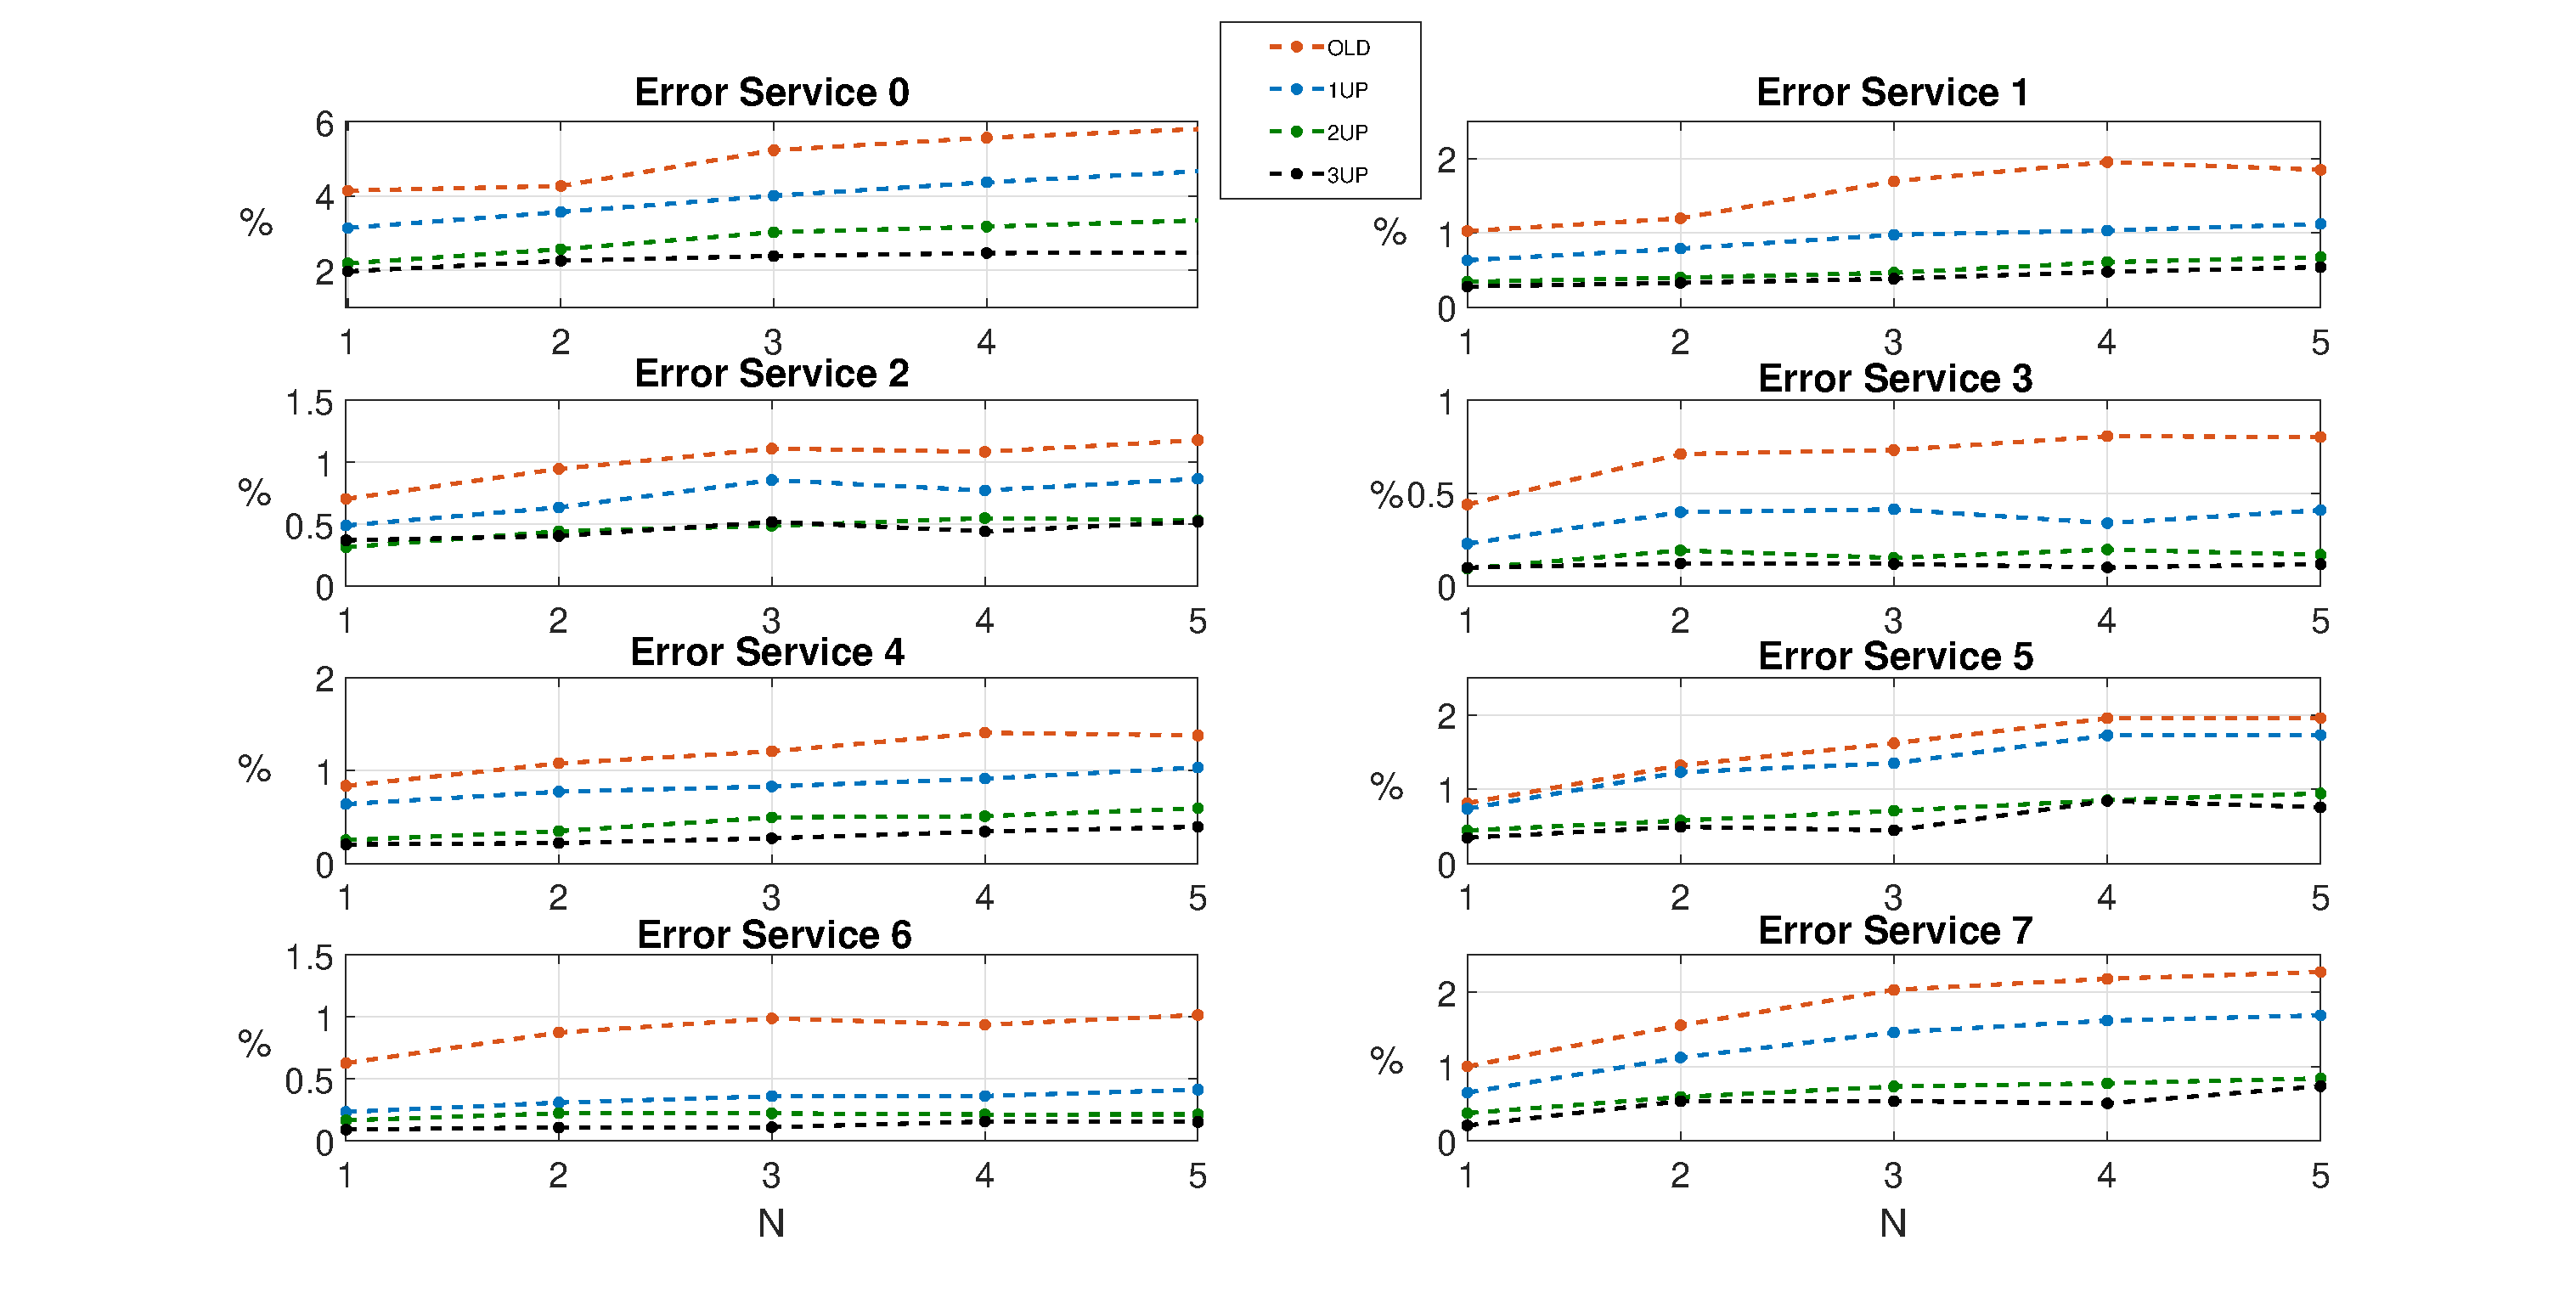
\includegraphics[trim={120 0 120 0}, width=1\linewidth]{figure/Error_Disturbance.eps}
	\caption{NRMSE of the disturbance predictive model over a time horizon of $N=5$.}
	\label{fig:{errorDist}}
\end{figure}
\begin{figure}[h!]
	\centering
	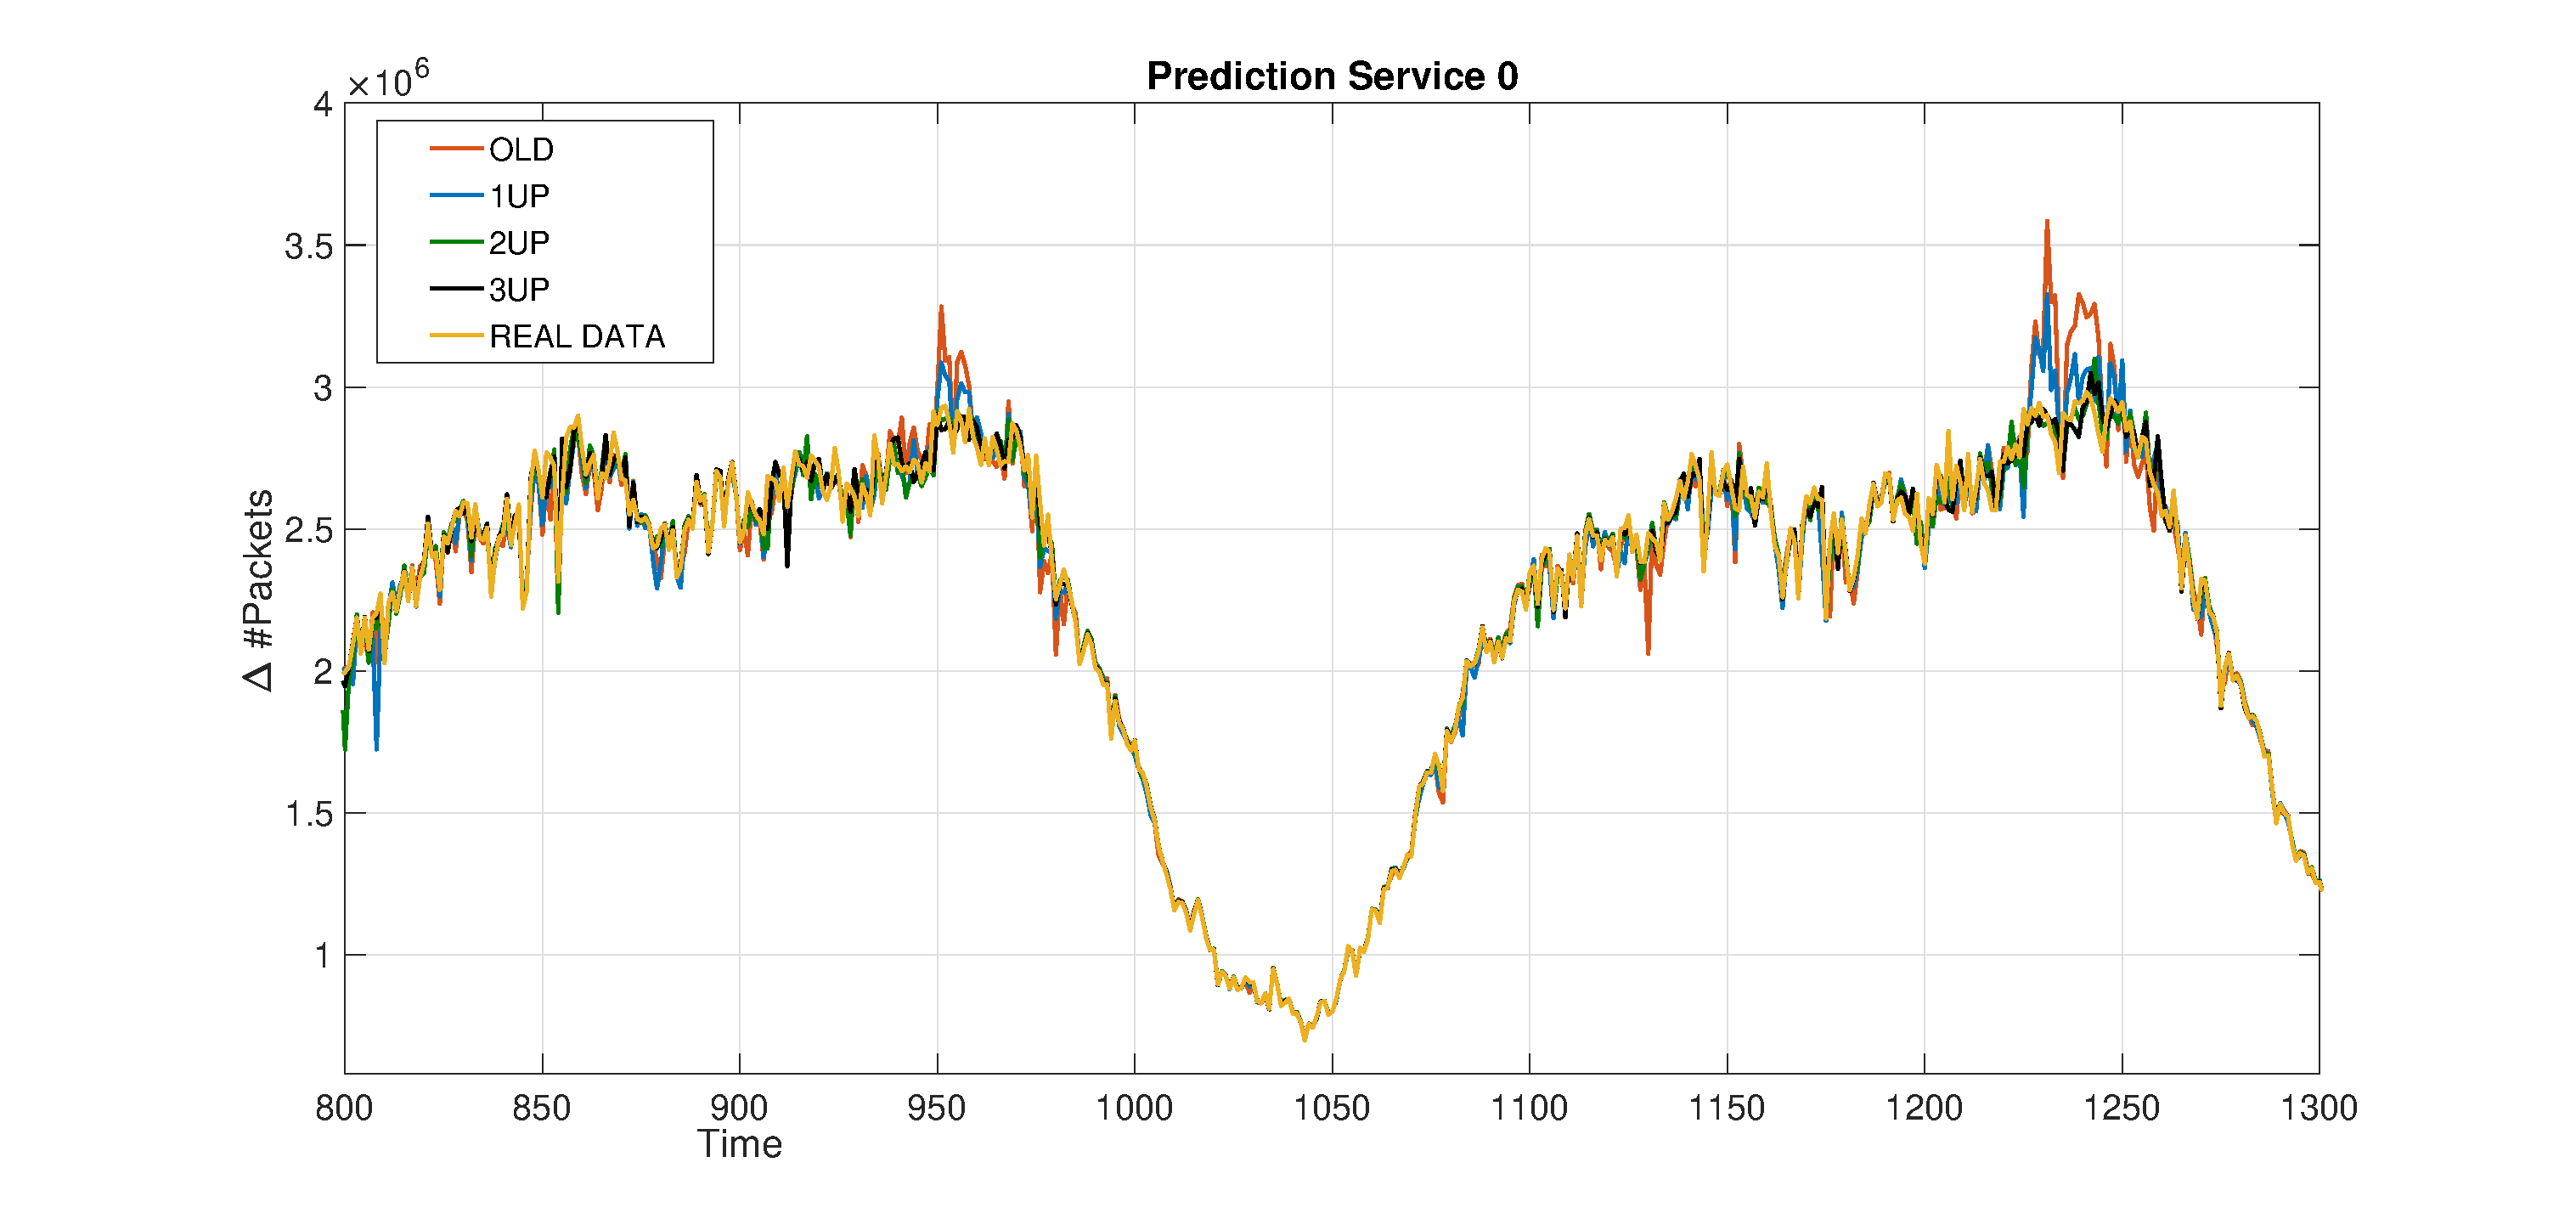
\includegraphics[trim={120 0 120 0}, width=1\linewidth]{figure/Error_Disturbance_Packets.eps}
	\caption{Comparison between the real traffic (YELLOW LINE) and the traffic prediction for the different models for Service 0.}
	\label{fig:{errorPack}}
\end{figure}

Figure \ref{fig:{errorDist}} shows the Normalised Root Mean Square Error (NRMSE) of the predictive model of the disturbance signals (one for each of the 8 DSCP indices) over a time horizon of $N=5$: the prediction error is worse for Service $0$ ($4-6\%$) since it includes the majority of the packets that transit through the switch. For other services the NRMSE is at most $2.2\%$ (Service 7) over all the predictive horizons. The improvement of the model accuracy when using larger (updated) data sets is evident, until a \textit{saturation} is reached and further data do not help to improve the model accuracy: the NRMSE significantly reduces and for Service 0 it is even halved. Figure \ref{fig:{errorPack}} plots, for Service $0$ and in a time window of $500$ samples (almost two days), the predictions of OLD, 1UP, 2UP and 3UP as well as the original data, and clearly highlights the better prediction of 2UP and 3UP with respect to OLD and 1UP.

%====================================================================================================

\subsection{Queues predictive model validation}

In this section we first compare the accuracy of our predictive models with Artificial Neural Networks. We recall that a neural network is a collection of algorithms that aim to identify underlying relations in a dataset: it consists of groups of connected neurons organized in layers, where the connections between neurons are modeled using weights. The signal produced with this linear composition is then fed into an activation function that is in general nonlinear. The reader is referred to \cite{NNstateOfART} and references therein for more details. A wide number of tools to build Neural Networks have been developed during recent years, e.g. \cite{tensorflow2015,chollet2015keras,openNN} just to mention a few: in this work we exploit the Deep Learning Toolbox of Matlab to compare predictive models based on NNs with the methodology proposed in this work, based on ARX combined RTs and RFs. We consider here just OLD as the learning dataset and chose a predictive horizon $N=5$.

To identify a RT (resp. RF) based predictive model of the queues we trained a Regression Tree (resp. a Random Forest) for each output and for each time horizon, with a total of $15$ trees (resp. $15$ forests each consisting of $30$ trees). The main parameters used for the identification algorithm (see Section \ref{secSwitchedModeling} and Problem \ref{pbLeastSquareProblem}) are summarized in Table \ref{tab:idPar}.  
\begin{table}[h!]
	\caption{Identification parameters}
	\centering
	\begin{tabular}{c c c c}
		\hline\hline
		Parameters & Value & Parameters & Values\\ 
		\hline
		N               & 5    & $f_{min}$   &-100 \\
		$\nu$        & 1     & $f_{max}$  &100  \\
		$\delta_x$ & 5     & $a_{min}$  &-100  \\
		$\delta_u$ & 5     & $a_{max}$ &100 \\
		$\delta_d$ & 5   & $b_{min}$  &0  \\
		Minleaf      & 13   & $b_{max}$ &10000  \\
		$|\Fij|$      & 30  &                   &\\
		\hline
	\end{tabular}
	\label{tab:idPar}
\end{table}
In particular, the regressive terms ($\delta_d$, $\delta_x$, $\delta_u$) and the minimum number of samples for each tree of each forest (MinLeaf) have been chosen, with a trial and error approach, considering that very small regressive horizons and very large values for MinLeaf may lead to inaccurate prediction (as they do not provide sufficient information on the past) but very large regressive horizons and very small values for MinLeaf also lead to inaccurate prediction (as they interpolate very old data that might negatively affect the results and produce overfitting).

Regarding specific parameters used for running NN, and for the sake of a fair comparison, we tuned them to obtain the best performance: in particular we considered shallow networks of 2 layers since depper networks did not improve the accuracy and, instead, have the negative effect of increasing the sensitivity of the accuracy with respect to the initial conditions of the weights. Among the many algorithms for optimizing the weights of the neurons we exploited the \textit{Scaled conjugate gradient back-propagation} described in \cite{Moller1990}, which provided the best accuracy with respect to our dataset. Regarding the activation functions, we used both the classical sigmoid function (\textit{LogSig}) and the Hyperbolic tangent sigmoid transfer function (\textit{TanSig}).
\begin{figure}[h!]
	\centering
	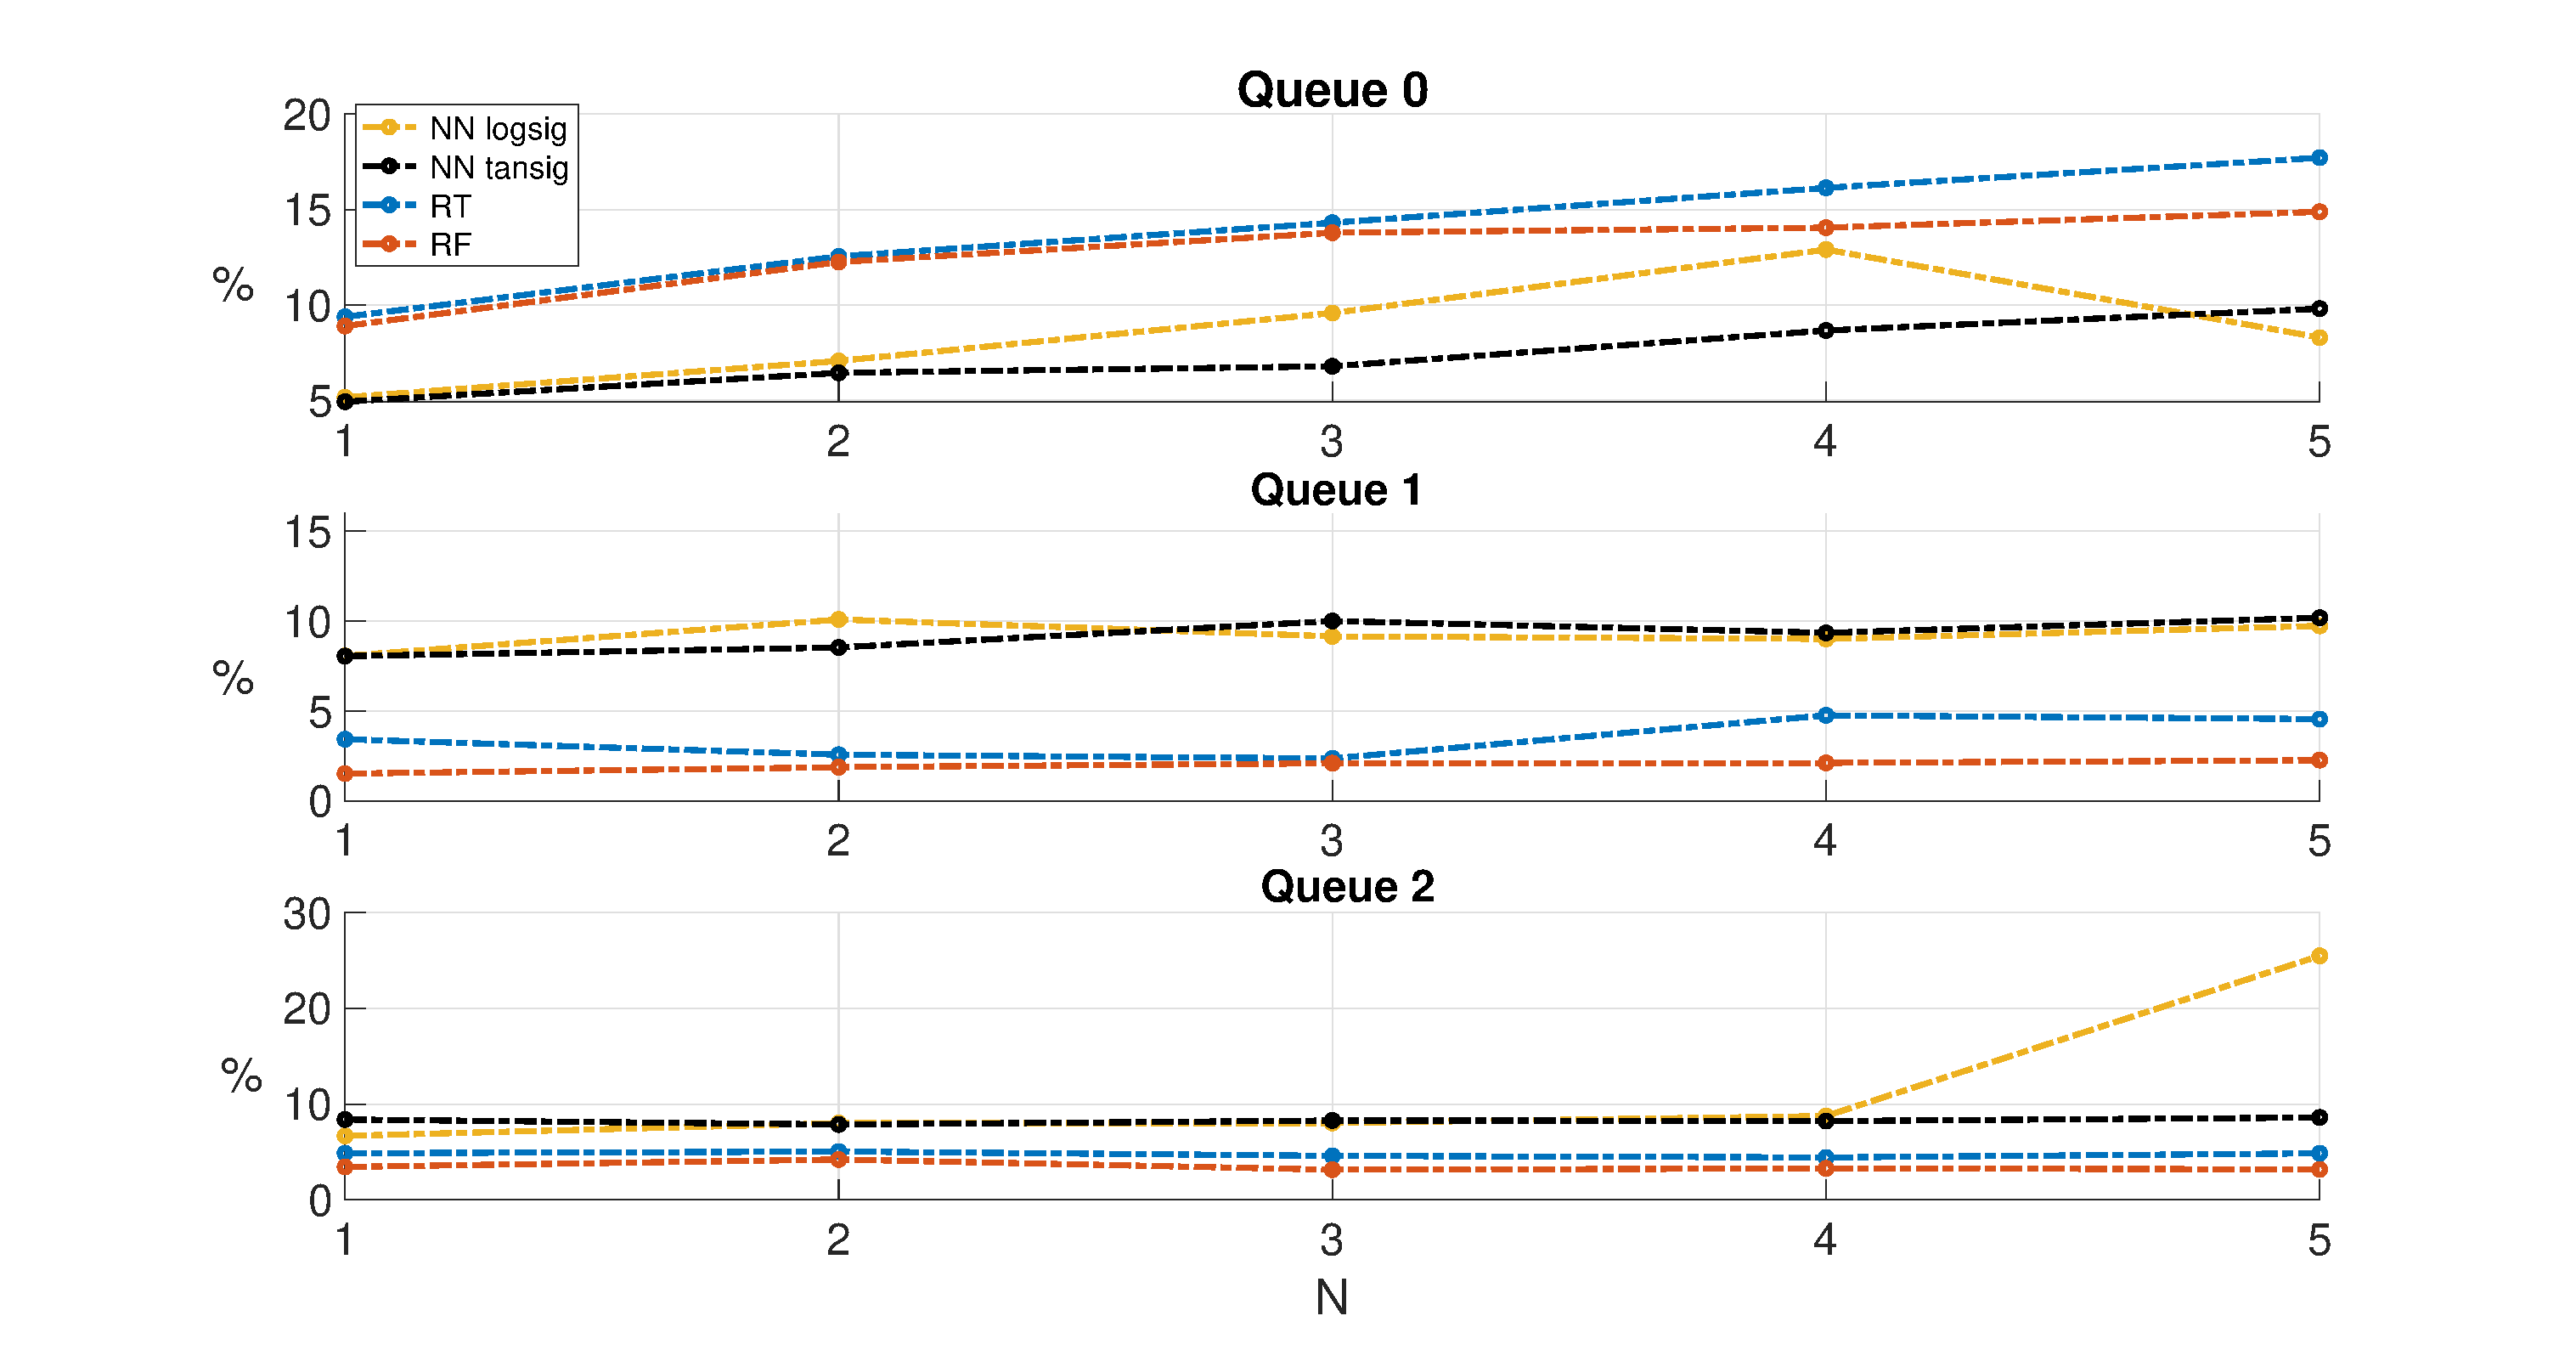
\includegraphics[trim={120 0 120 0},width=0.9\linewidth]{figure/NRMSENNvsRTvsRF.eps}
	\vspace{-0.2cm}
	\caption{NRMSE, up to $N=5$ and for each priority class, for RT (blue), RF (red), NN with sigmoids as activation function (yellow) and NN with hyperbolic tangent as activation function (black).}
	\label{fig:{NRMSE}}
\end{figure}

As a metric of the prediction accuracy we compared in Figure \ref{fig:{NRMSE}} the Normalized Root Mean Square Errors (NRMSE) of the different identification approaches for each priority class and over a horizon up to $N=5$. Regarding queue $0$ (Default) NNs perform better than RT and RF, but in queues $1$ (Premium) and $2$ (Gold), characterised by higher priority, RF provides the best performance. Queue $0$ is characterised by a larger NRMSE with all identification techniques: this is due to the fact that, having the lowest priority, it suffers more packet losses and this can negatively affect the prediction accuracy. Our validation emphasizes that RTs, even thought very simple and fast to compute, are often affected by overfitting and variance issues, i.e. small variations of the training data result in large variations of the tree structure and, consequently, of the predictions. Regarding NNs, they provide a less accurate model in 2 cases over 3. Indeed, by analyzing the dataset distribution (see Figure \ref{fig:{datadistribution}}), we noticed a peculiar regular grid pattern that can be very well approximated by hyper-rectangles: since RTs and RFs base their prediction on hyper-rectangular dataset partitions, the better performance with respect to NNs is reasonable.
\begin{figure}[h!]
	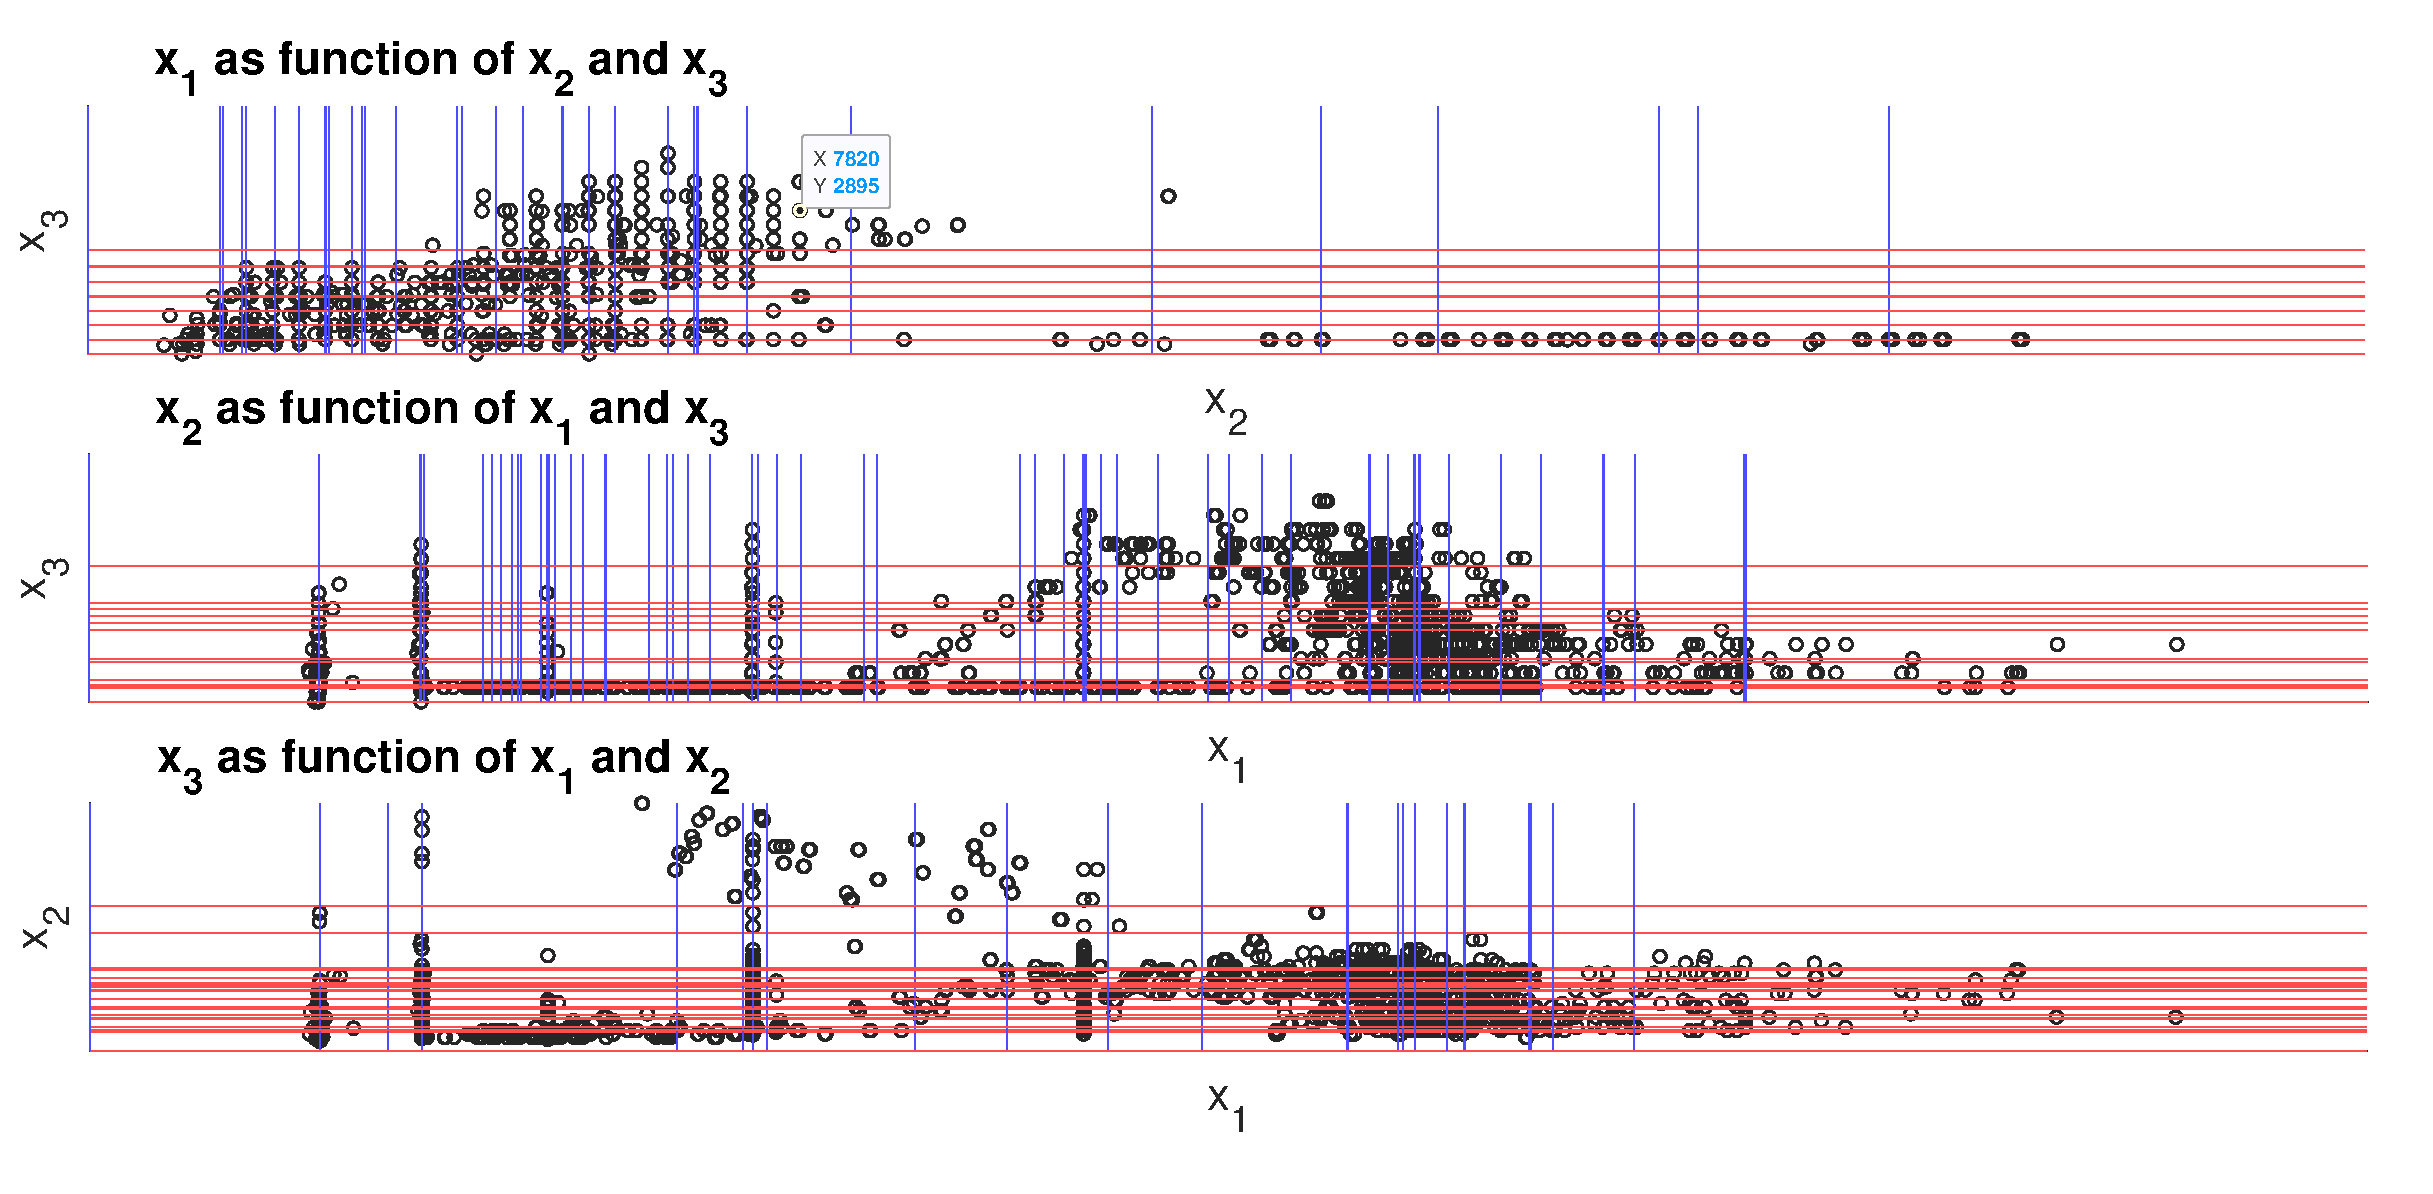
\includegraphics[width=\linewidth]{figure/datadistribution.eps}
	\caption{Grid pattern emerged from dataset distribution.}
	\label{fig:{datadistribution}}
\end{figure}
For queue 0, even thought NNs perform better, we need to remark that their predictive model is based on nonlinear functions: this makes the derived model impractical for real-time control as the corresponding MPC formulation turns into a nonlinear optimization problem, for which there is no approach that can guarantee neither a global optimal solution nor a reasonable computation time. In addition to this, even obtaining a closed mathematical form of the predictive function of a Neural Network starting from neurons and weitghts is not always an easy task, because of the highly nonlinear interconnections between the different layers. For all these reasons we decided to only use from now on RF-based models, which provide the best choice both from the accuracy and the computational complexity points of view. In the following we illustrate the effect of iterative dataset updates in the prediction accuracy, both with and without knowledge of the future disturbances.
\begin{figure}[th!]
	\centering
	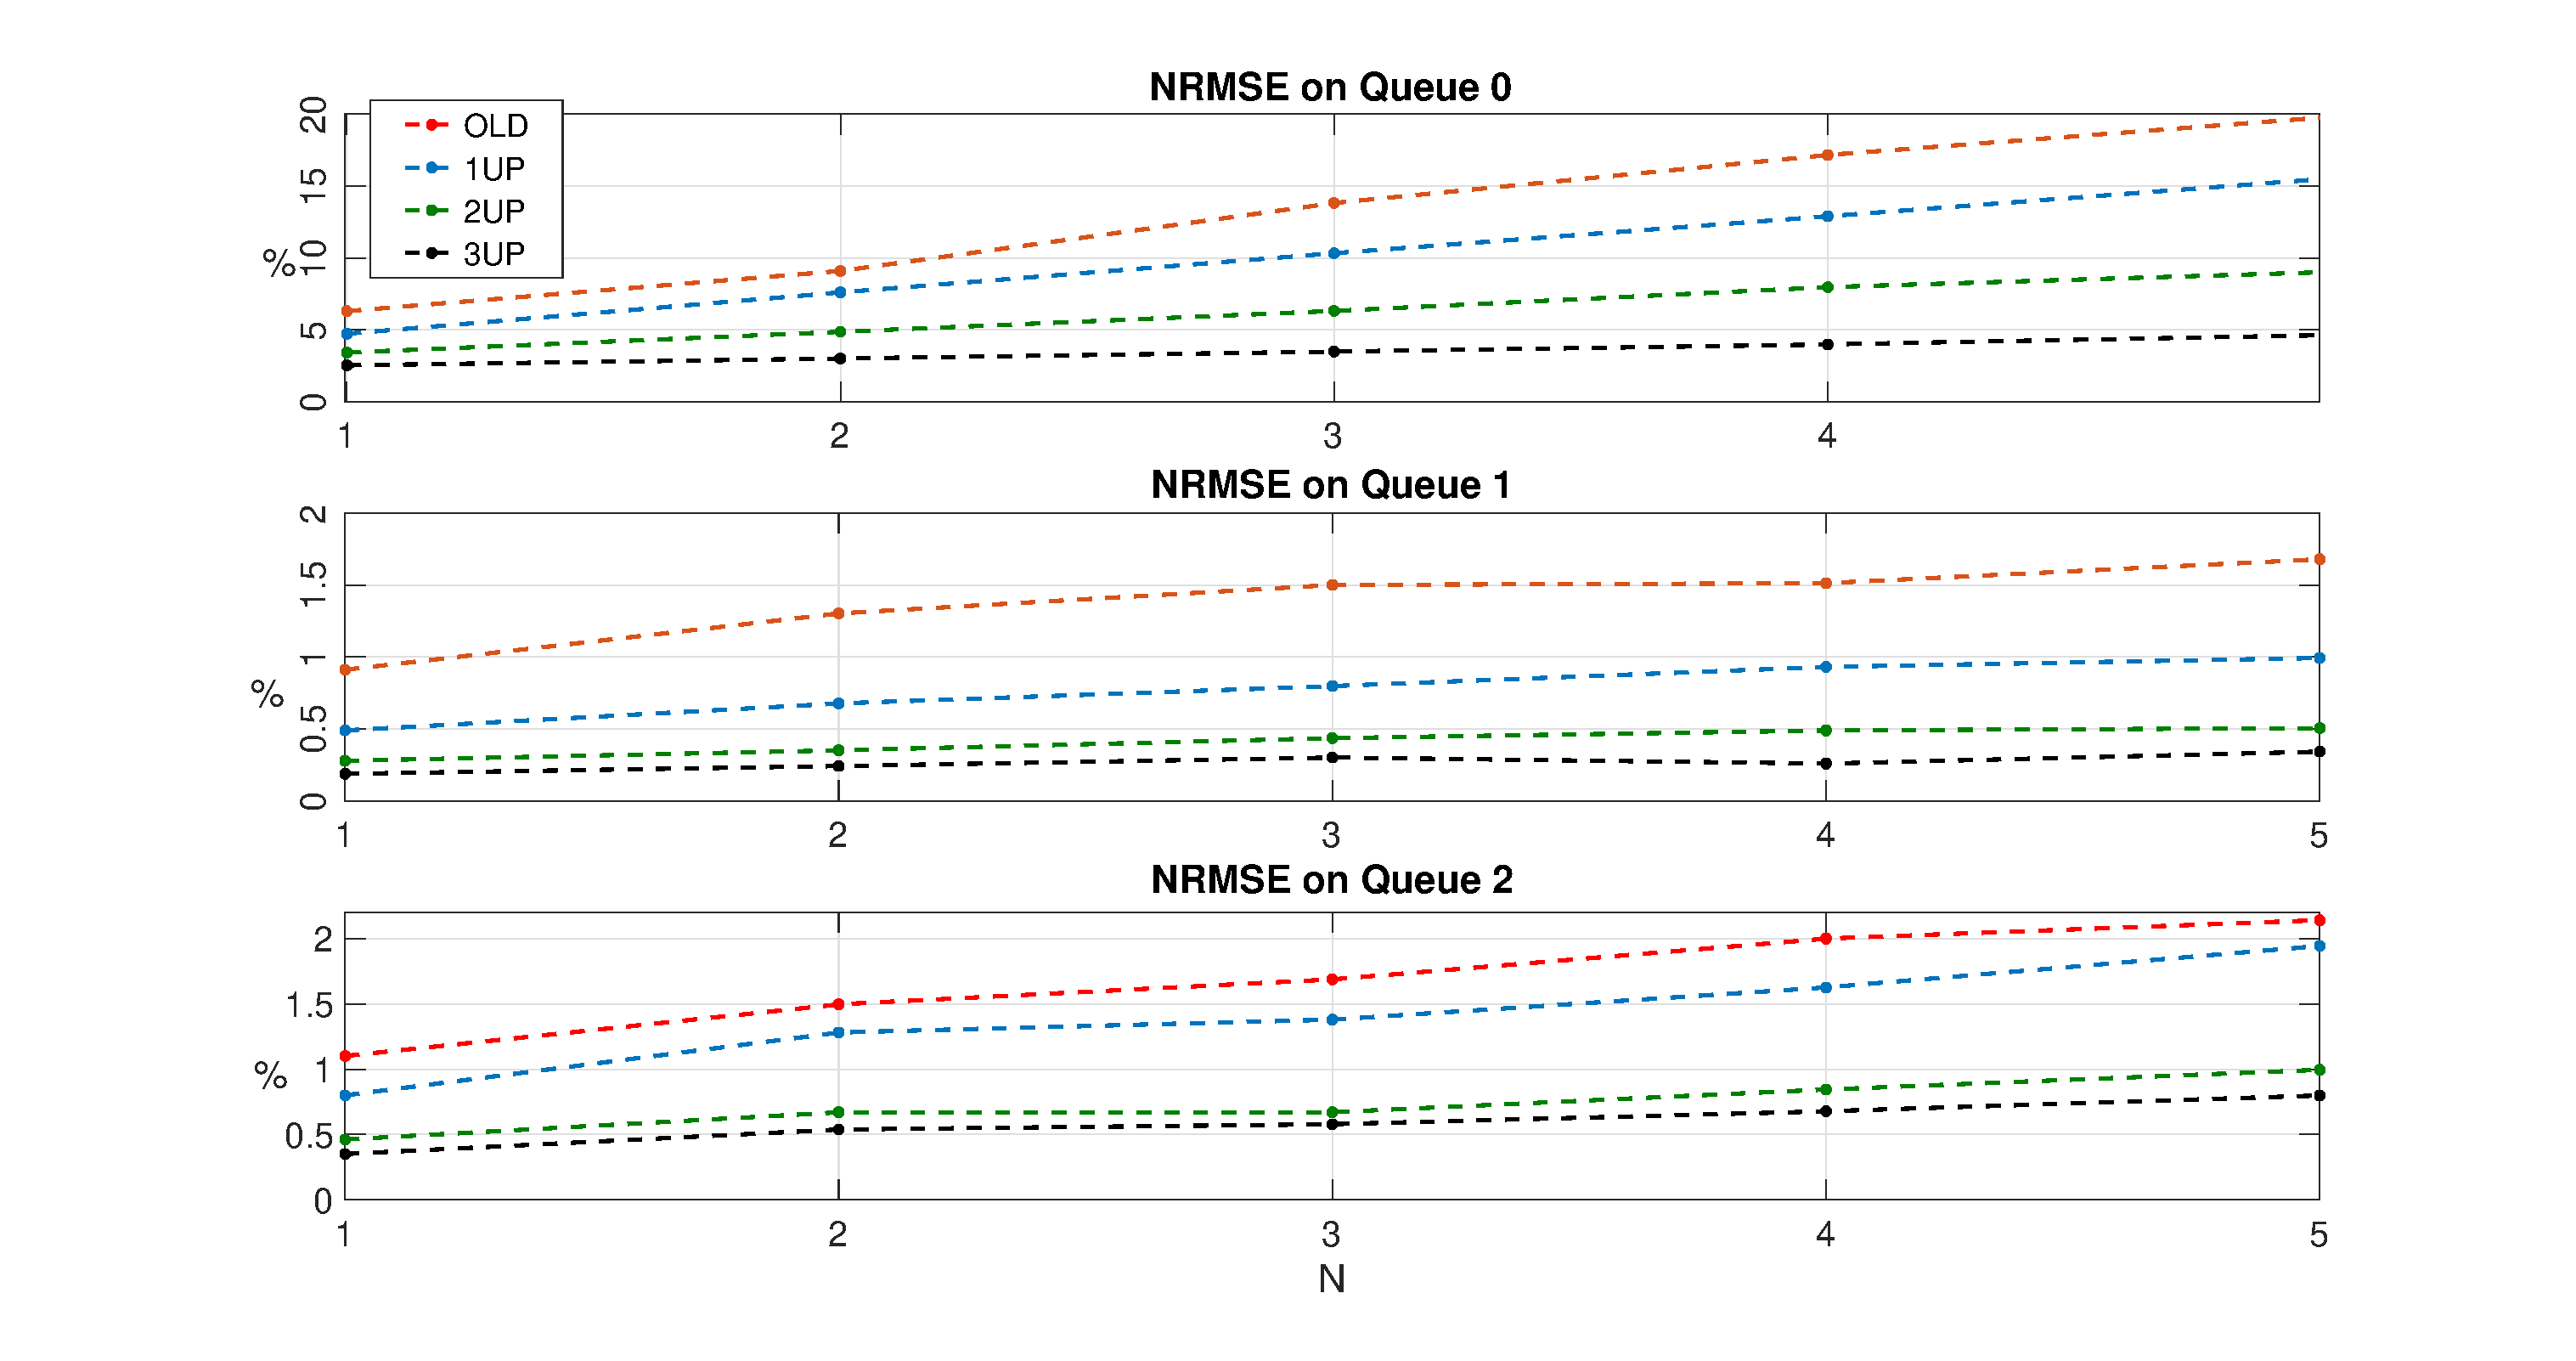
\includegraphics[trim={120 0 120 0}, width=0.9\linewidth]{figure/Error_State.eps}
	\caption{NRMSE of the queues output predictive model over a time horizon of $N=5$, without knowledge of the future disturbances}
	\label{fig:{stateNRMSE}}
\end{figure}
\begin{figure}[th!]
	\centering
	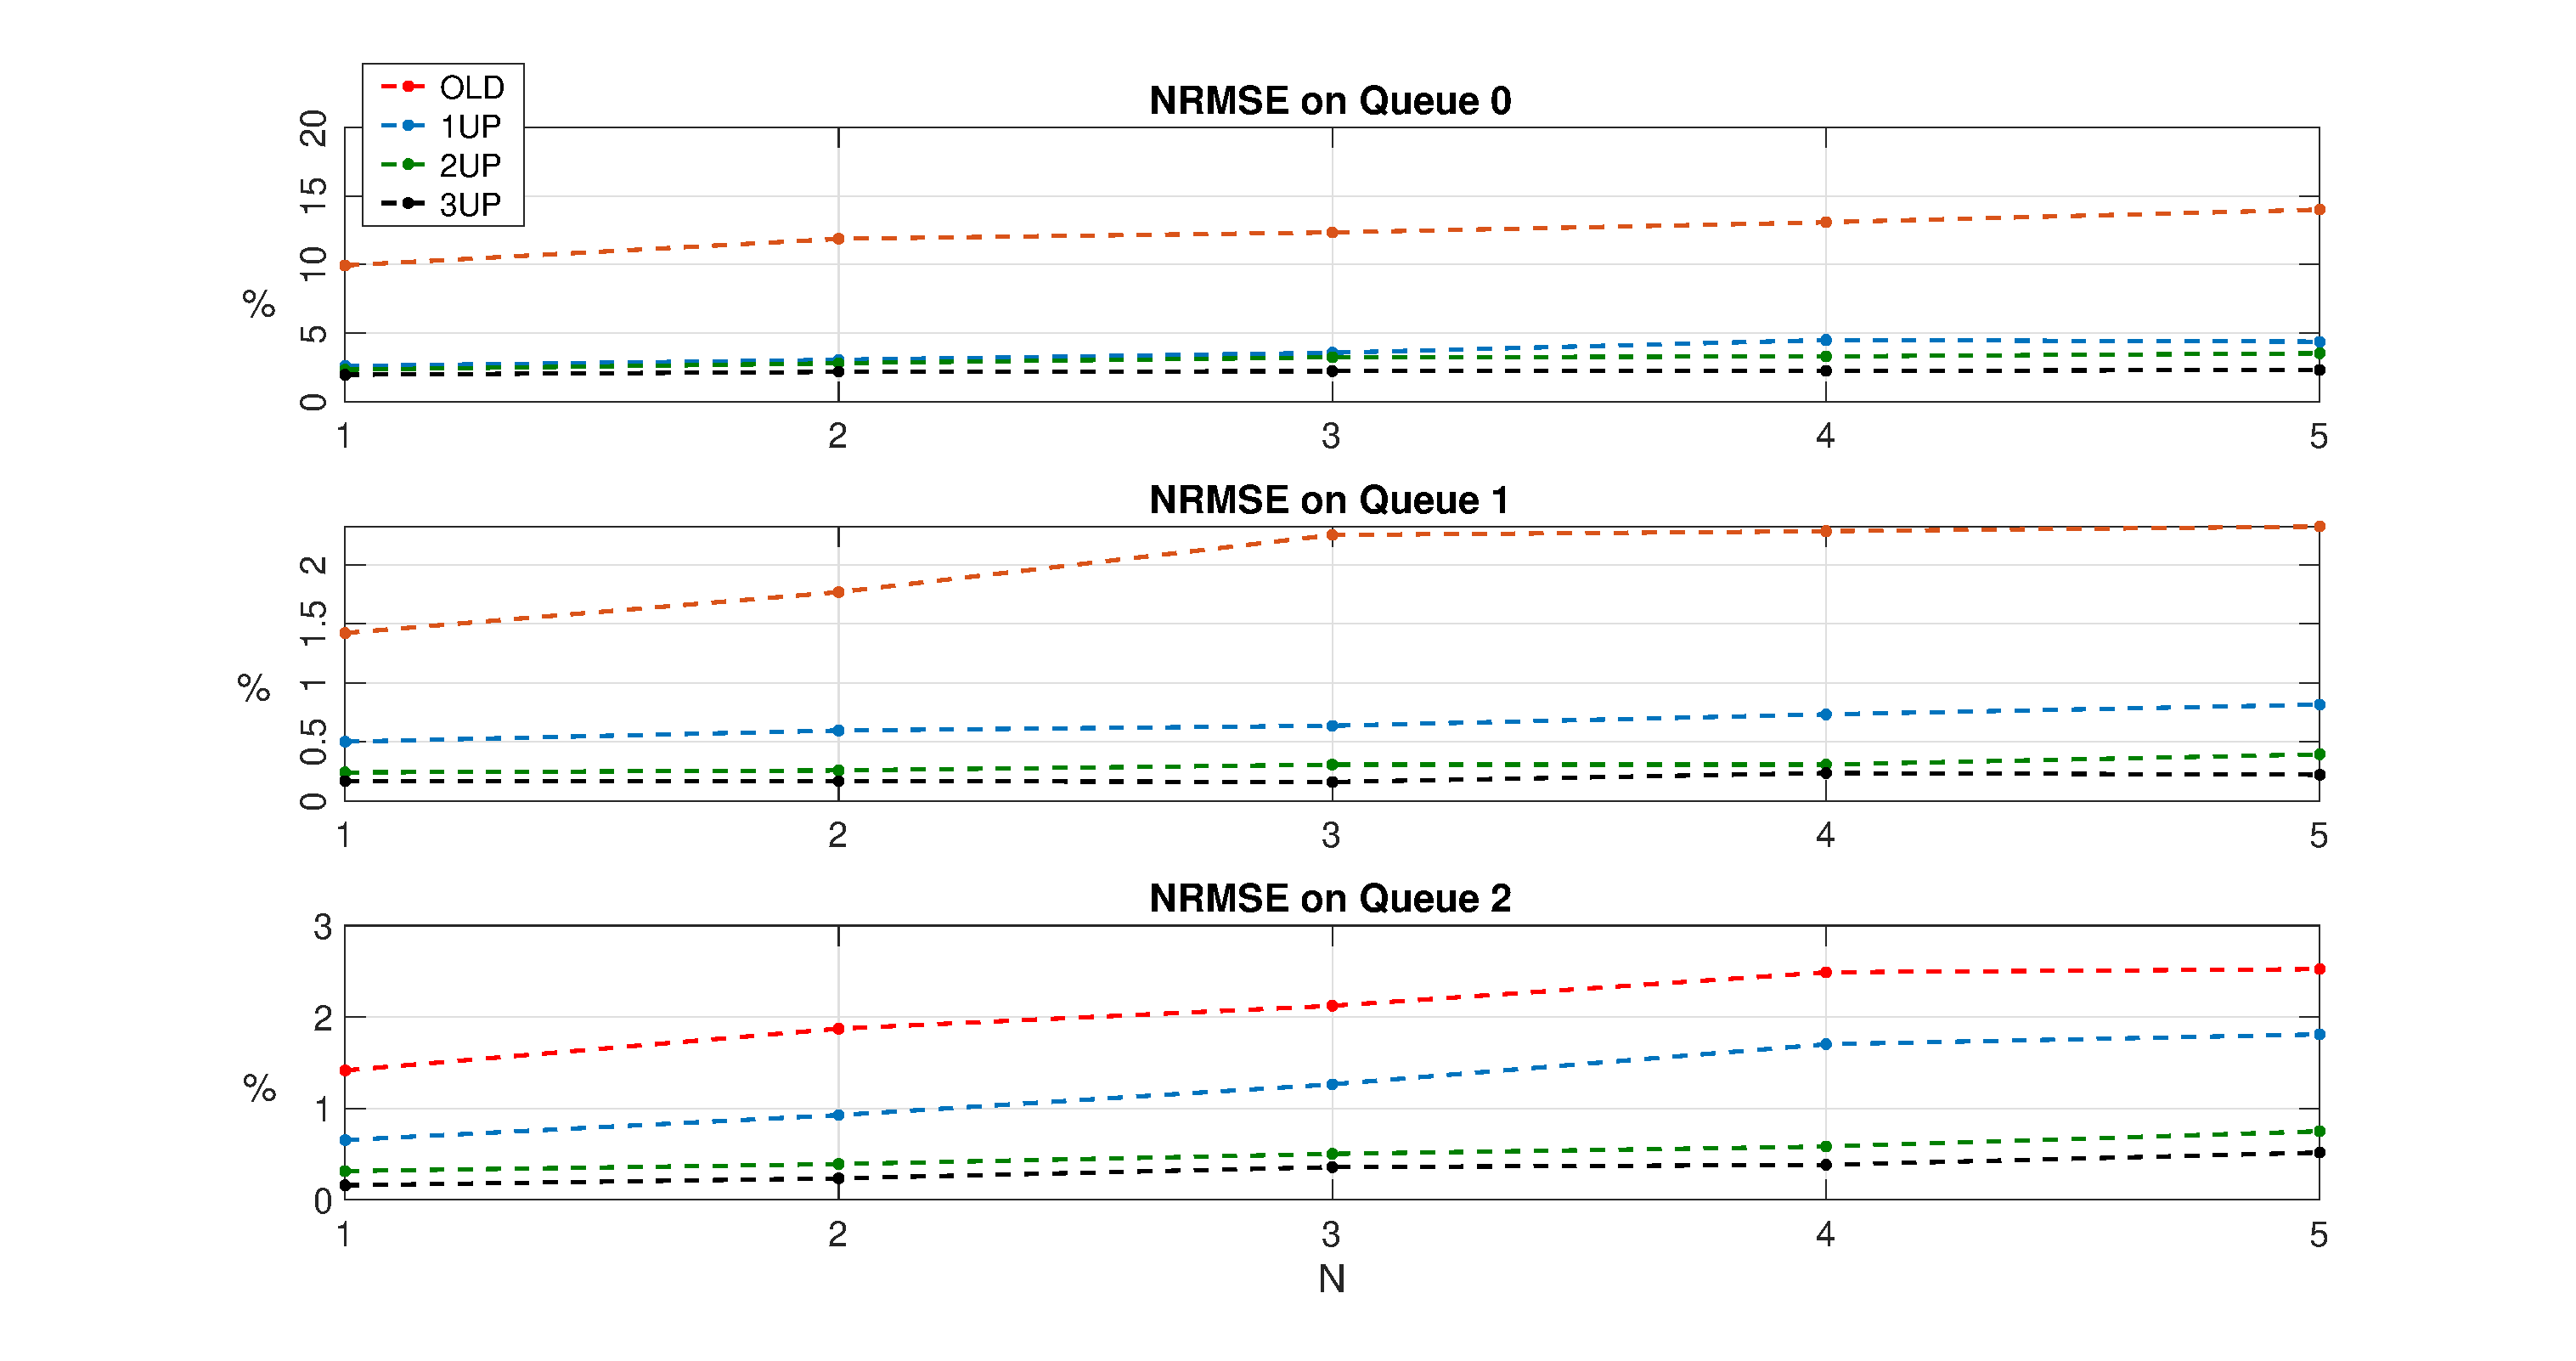
\includegraphics[trim={120 0 120 0}, width=0.9\linewidth]{figure/Error_State_ddM4.eps}
	\caption{NRMSE of the queues output predictive model over a time horizon of $N=5$, with knowledge of the 4-steps future disturbances}
	\label{fig:{stateNRMSEddM4}}
\end{figure}

Figure \ref{fig:{stateNRMSE}} and Figure \ref{fig:{stateNRMSEddM4}} plot the NRMSEs respectively without and with knowledge of the future disturbances. The assumption of future disturbance forecast, as expected, provides much better prediction accuracy. The positive effect of updated data sets is also clear, providing accuracy improvements up to $50 \%$: as will be also discussed in the next section, the most relevant prediction accuracy improvement takes place moving from OLD to 1UP or from 1UP to 2UP, while the 3UP model does not improve much.

\begin{remark}
We wish to highlight that in our simulations we generated data without major modifications of the traffic daily pattern: for this reason enriching the data set converges to a saturation of the model accuracy, as discussed above. Nevertheless, the capability of our methodology to iteratively learn from new data is fundamental as, in real life, changes in the traffic patterns do occur, and model updates are necessary to maintain the model accuracy and the control performance. 
\end{remark}

%====================================================================================================

\subsection{Control performance}\label{sec:control_performance}

In this section we setup a control loop where the (Mininet) network emulator and the (Ryu) controller run in two different computers, and synchronize/exchange data using a shared file. Namely, our SW controller module is, in principle, ready to be directly used on a real SDN-based network, with just some minor modifications in the data exchange with the switch devices. The controller implements MPC using the predictive models validated in the previous sections: at each time step, it solves Problem \ref{pbMPC} and optimally updates the bandwidth of the different queues. The cost matrices $Q$ and $R$ of Problem \ref{pbMPC} respectively weight the output $y(k)$ of the system (i.e. the packet transmission rate for each queue) and the control input $u(k)$ (i.e. the bandwidth assigned to each queue). Since $R$ is required to be positive definite but it makes no sense assigning a penalty to the choice of $u(k)$, we define $R=10^{-5} \cdot \mathbb I$, where the identity matrix $\mathbb I$ multiplies a very small value. Matrix $Q = diag(1,10^4,10)$ has been assigned as a diagonal matrix, where the choice of the different diagonal components is related to the priority level of each queue. The remaining constraints of Problem \ref{pbMPC} are reported in Table \ref{tab:contPar}.
%The parameters used in the constraints described in Problem \ref{pbMPC} are reported in Table \ref{tab:contPar} and the weights matrices considered in the optimisation cost are: $Q=diag([1,1000,10])$ and $R=10^{-5} \mathbb{I}_3$.
\begin{table}[h!]
	\caption{Constraints in Problem \ref{pbMPC}}
	\centering
	\begin{tabular}{l c l c}
		\hline\hline
		Parameters                                & Value               & Parameters                 & Values       \\ 
		\hline
		$\Delta u_1^\mathrm{min}$     & 1                   & $\Delta u_1^\mathrm{max}$  & 30           \\
		$\Delta u_2^\mathrm{min}$     & 20                  & $\Delta u_2^\mathrm{max}$  & 30           \\
		$\Delta u_3^\mathrm{min}$     & 20                  & $\Delta u_3^\mathrm{max}$  & 20           \\
		$u_1^\mathrm{min} $             & 10                  & $u_1^\mathrm{max} $        & 45           \\
		$u_2^\mathrm{min} $            & 55                  & $u_2^\mathrm{max} $        & 80           \\
		$u_3^\mathrm{min} $            & 80                  & $u_3^\mathrm{max} $        & 100          \\
		
		\hline
	\end{tabular}
	\label{tab:contPar}
\end{table}
In what follows we validate the control performance both without and with knowledge of the future disturbances. The value of $x_\mathrm{ref}$ in the optimization problem represents the reference value we chose for tracking system output: indeed, as we wish to minimize packet losses, we minimize the difference between the packets received by the hosts $d(k)$ and those transmitted by the queues $y(k)$ over the horizon $N$. In case we have no knowledge of future disturbances, we consider $x_\mathrm{ref}$ equal to the current disturbance  measurement $d(k)$ and constant over all the predictive horizon; if instead we have knowledge of future disturbances, we consider $x_\mathrm{ref}$ equal to such future disturbances. In this section we decided to only compare models OLD, 1UP and 2UP, since model 3UP does not provide any substantial improvement. 

 \begin{figure}[h!]
	\centering
	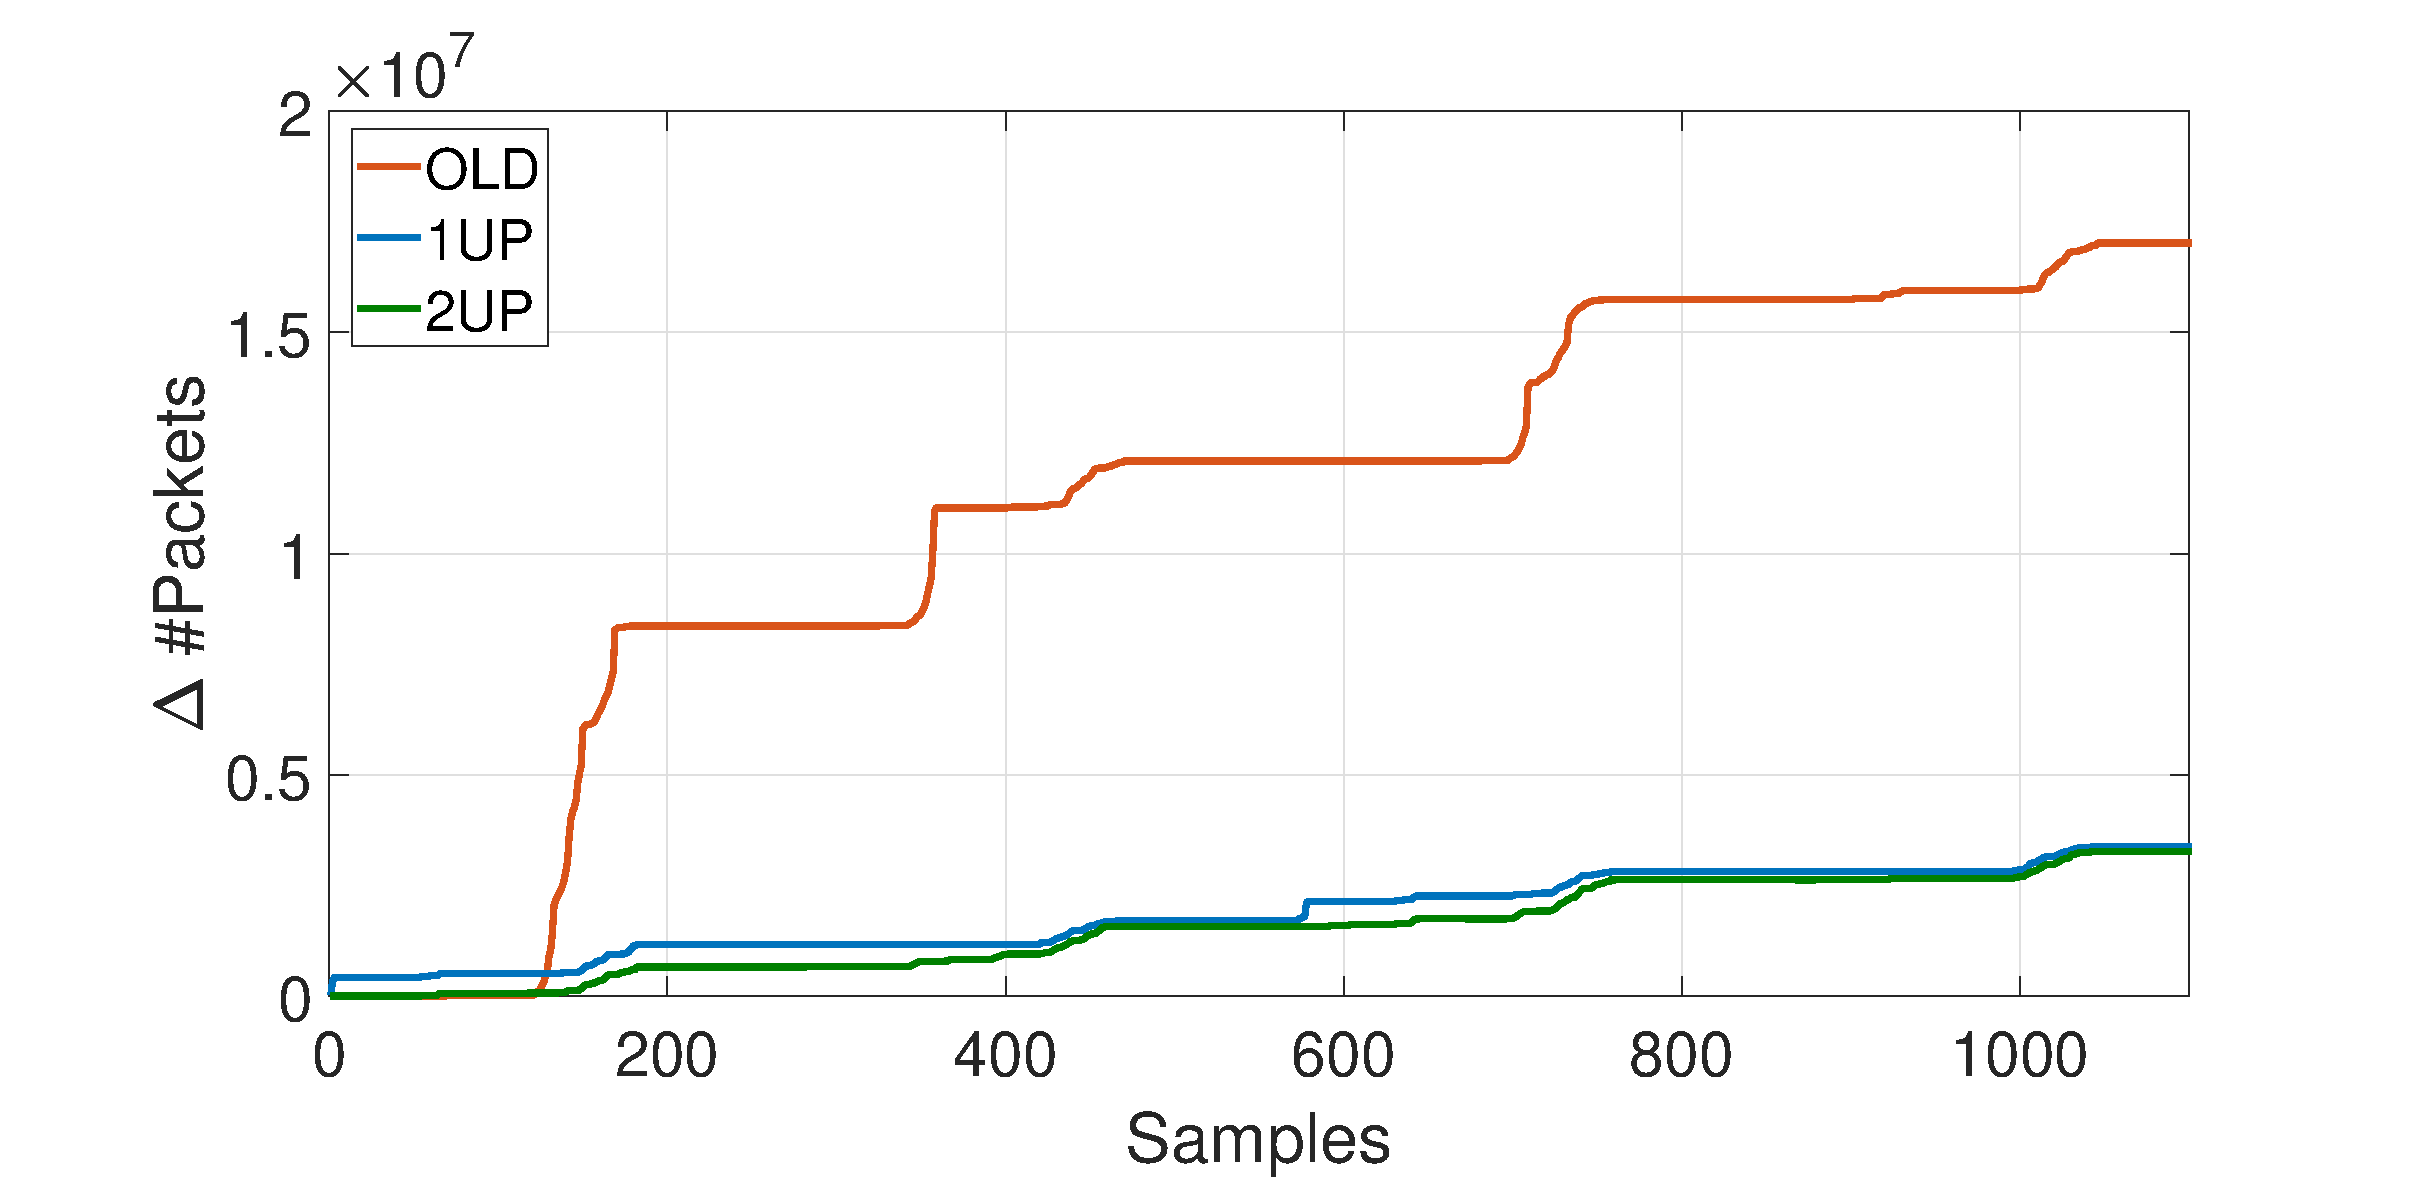
\includegraphics[trim={120 0 120 0}, width=0.9\linewidth]{figure/cumPL1.eps}
	\caption{Cumulative Packet Losses without knowledge of the future disturbance.}
	\label{fig:{MPC1}}
\end{figure}
\begin{figure}[h!]
	\centering
	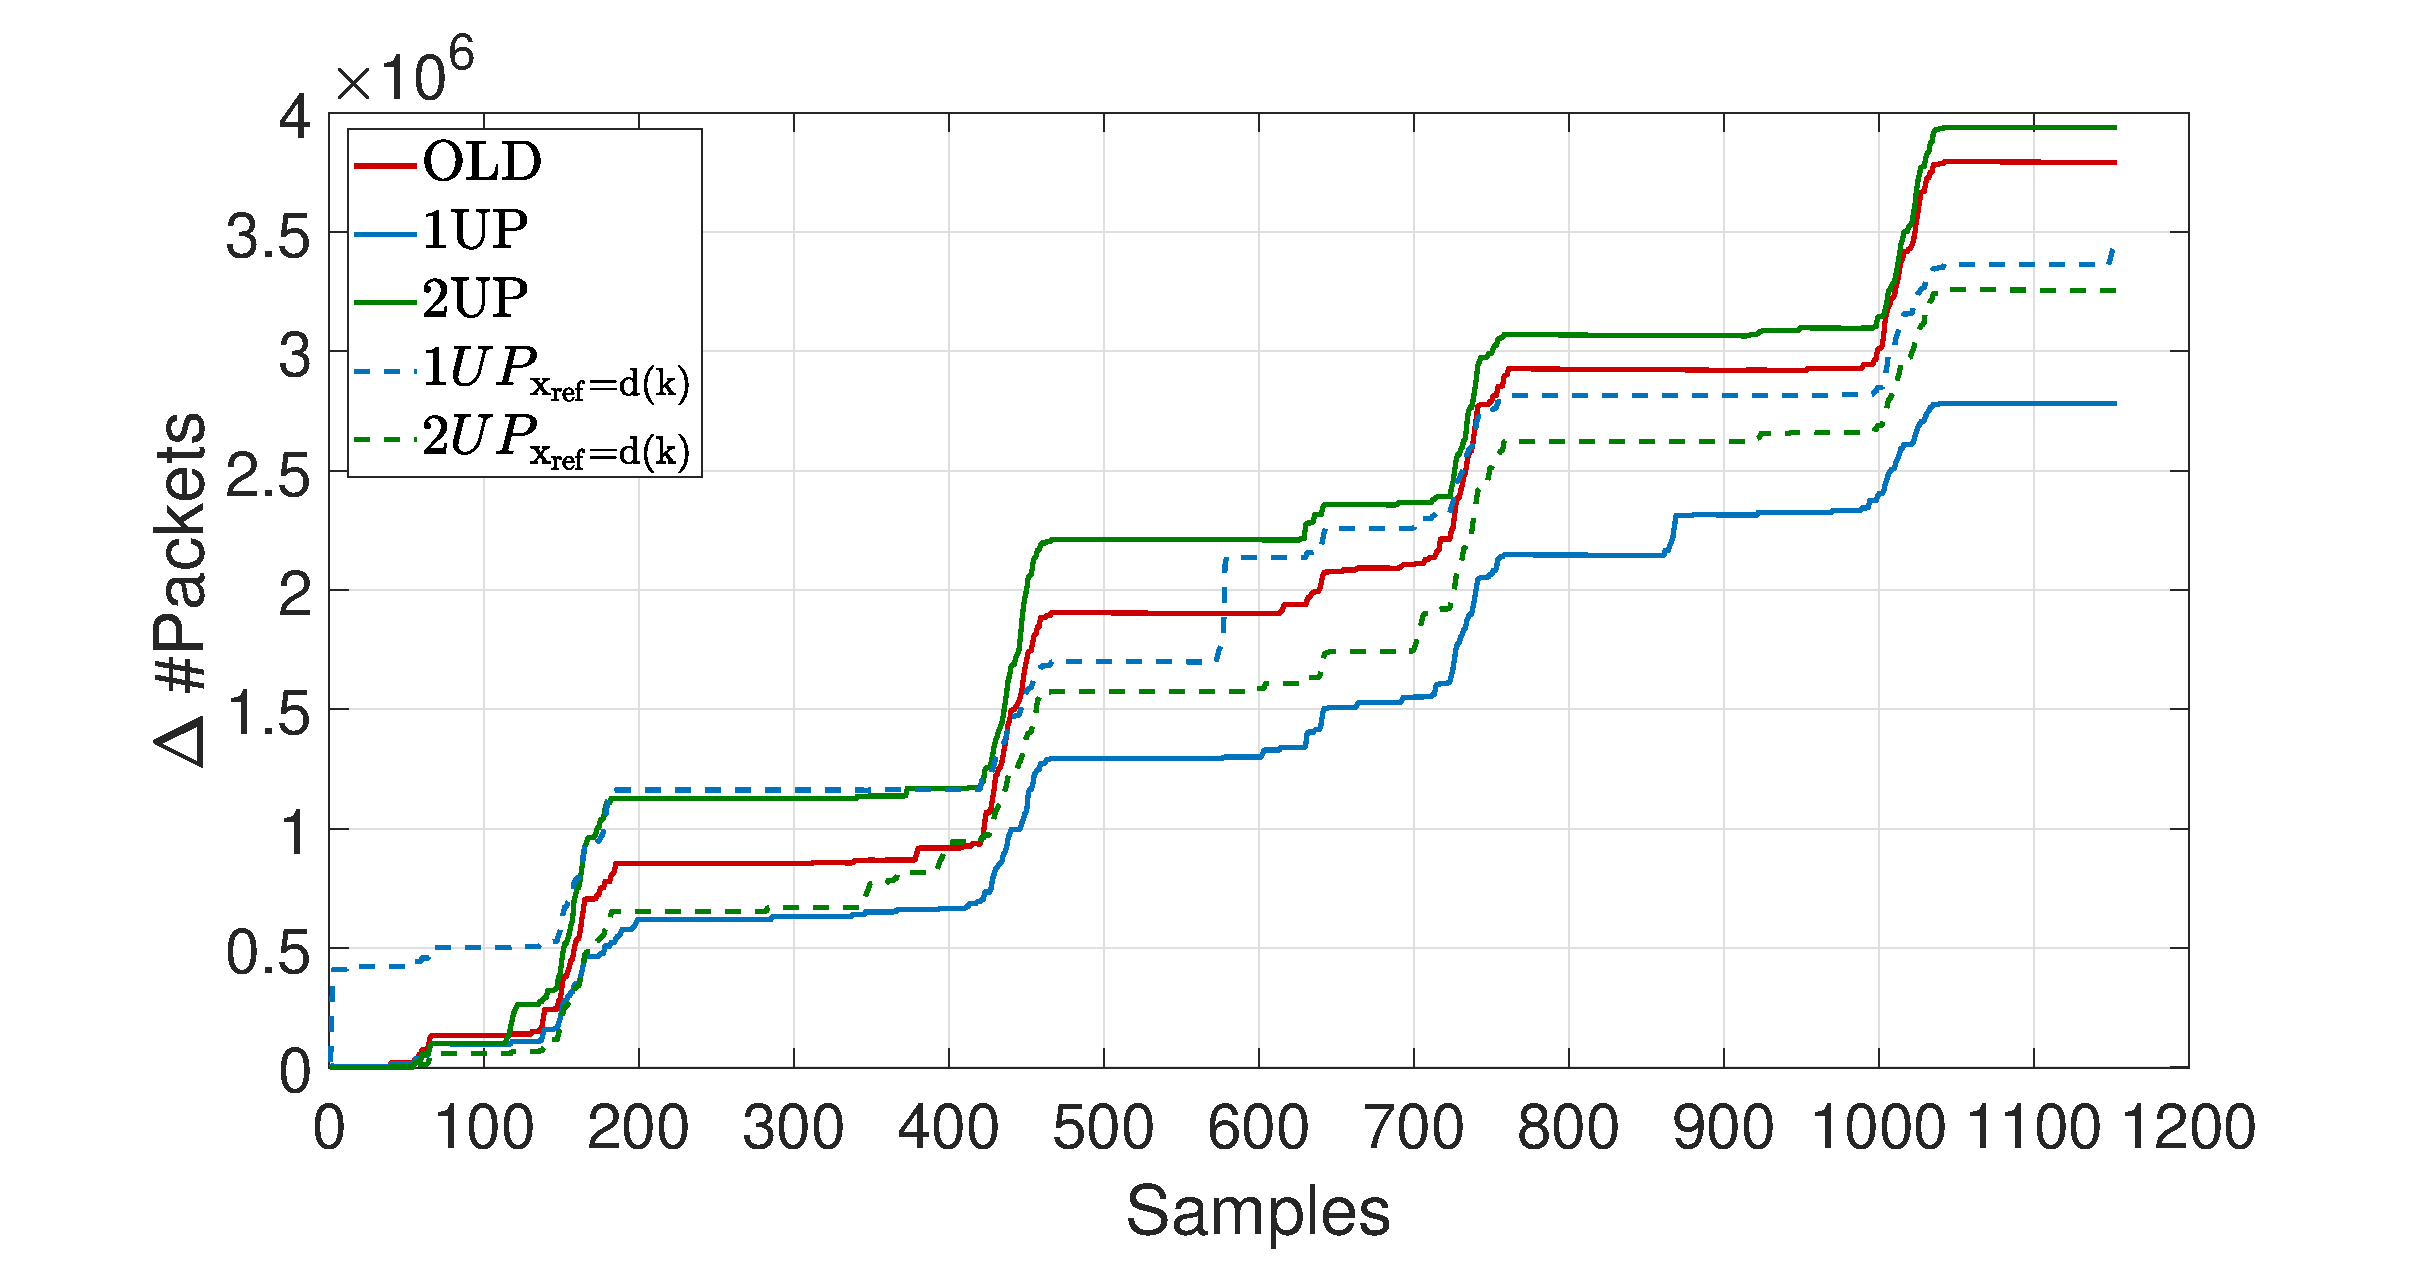
\includegraphics[trim={120 0 120 0},width=0.9\linewidth]{figure/cumPL_Total.eps}
	\caption{Comparison between Cumulative Packet Losses with (solid lines)  and without (dashed lines) knowledge of the future disturbance.}
	\label{fig:{MPC2}}
\end{figure}
 Figures \ref{fig:{MPC1}} and \ref{fig:{MPC2}} plot the cumulative packet losses respectively without and with knowledge of the future disturbances. The packet loss rate when the control is performed exploiting the OLD model and without disturbance forecast is around $123\%$ larger than all other cases (and, of course, incomparably smaller than the static control case \cite{Notiziario}). It is also clear from the plots that 1UP and 2UP without disturbance forecast and OLD, 1UP and 2UP with disturbance forecast provide very similar performance. Our interpretation is that OLD models without disturbance forecast have not enough information to provide good accuracy, but they can be easily improved either with a data set update (which however requires $10$ days for 1UP and $20$ days for 2UP of additional data) or using a predictive disturbance model.

\begin{figure}[h!]
\centering
\subfigure[a][]{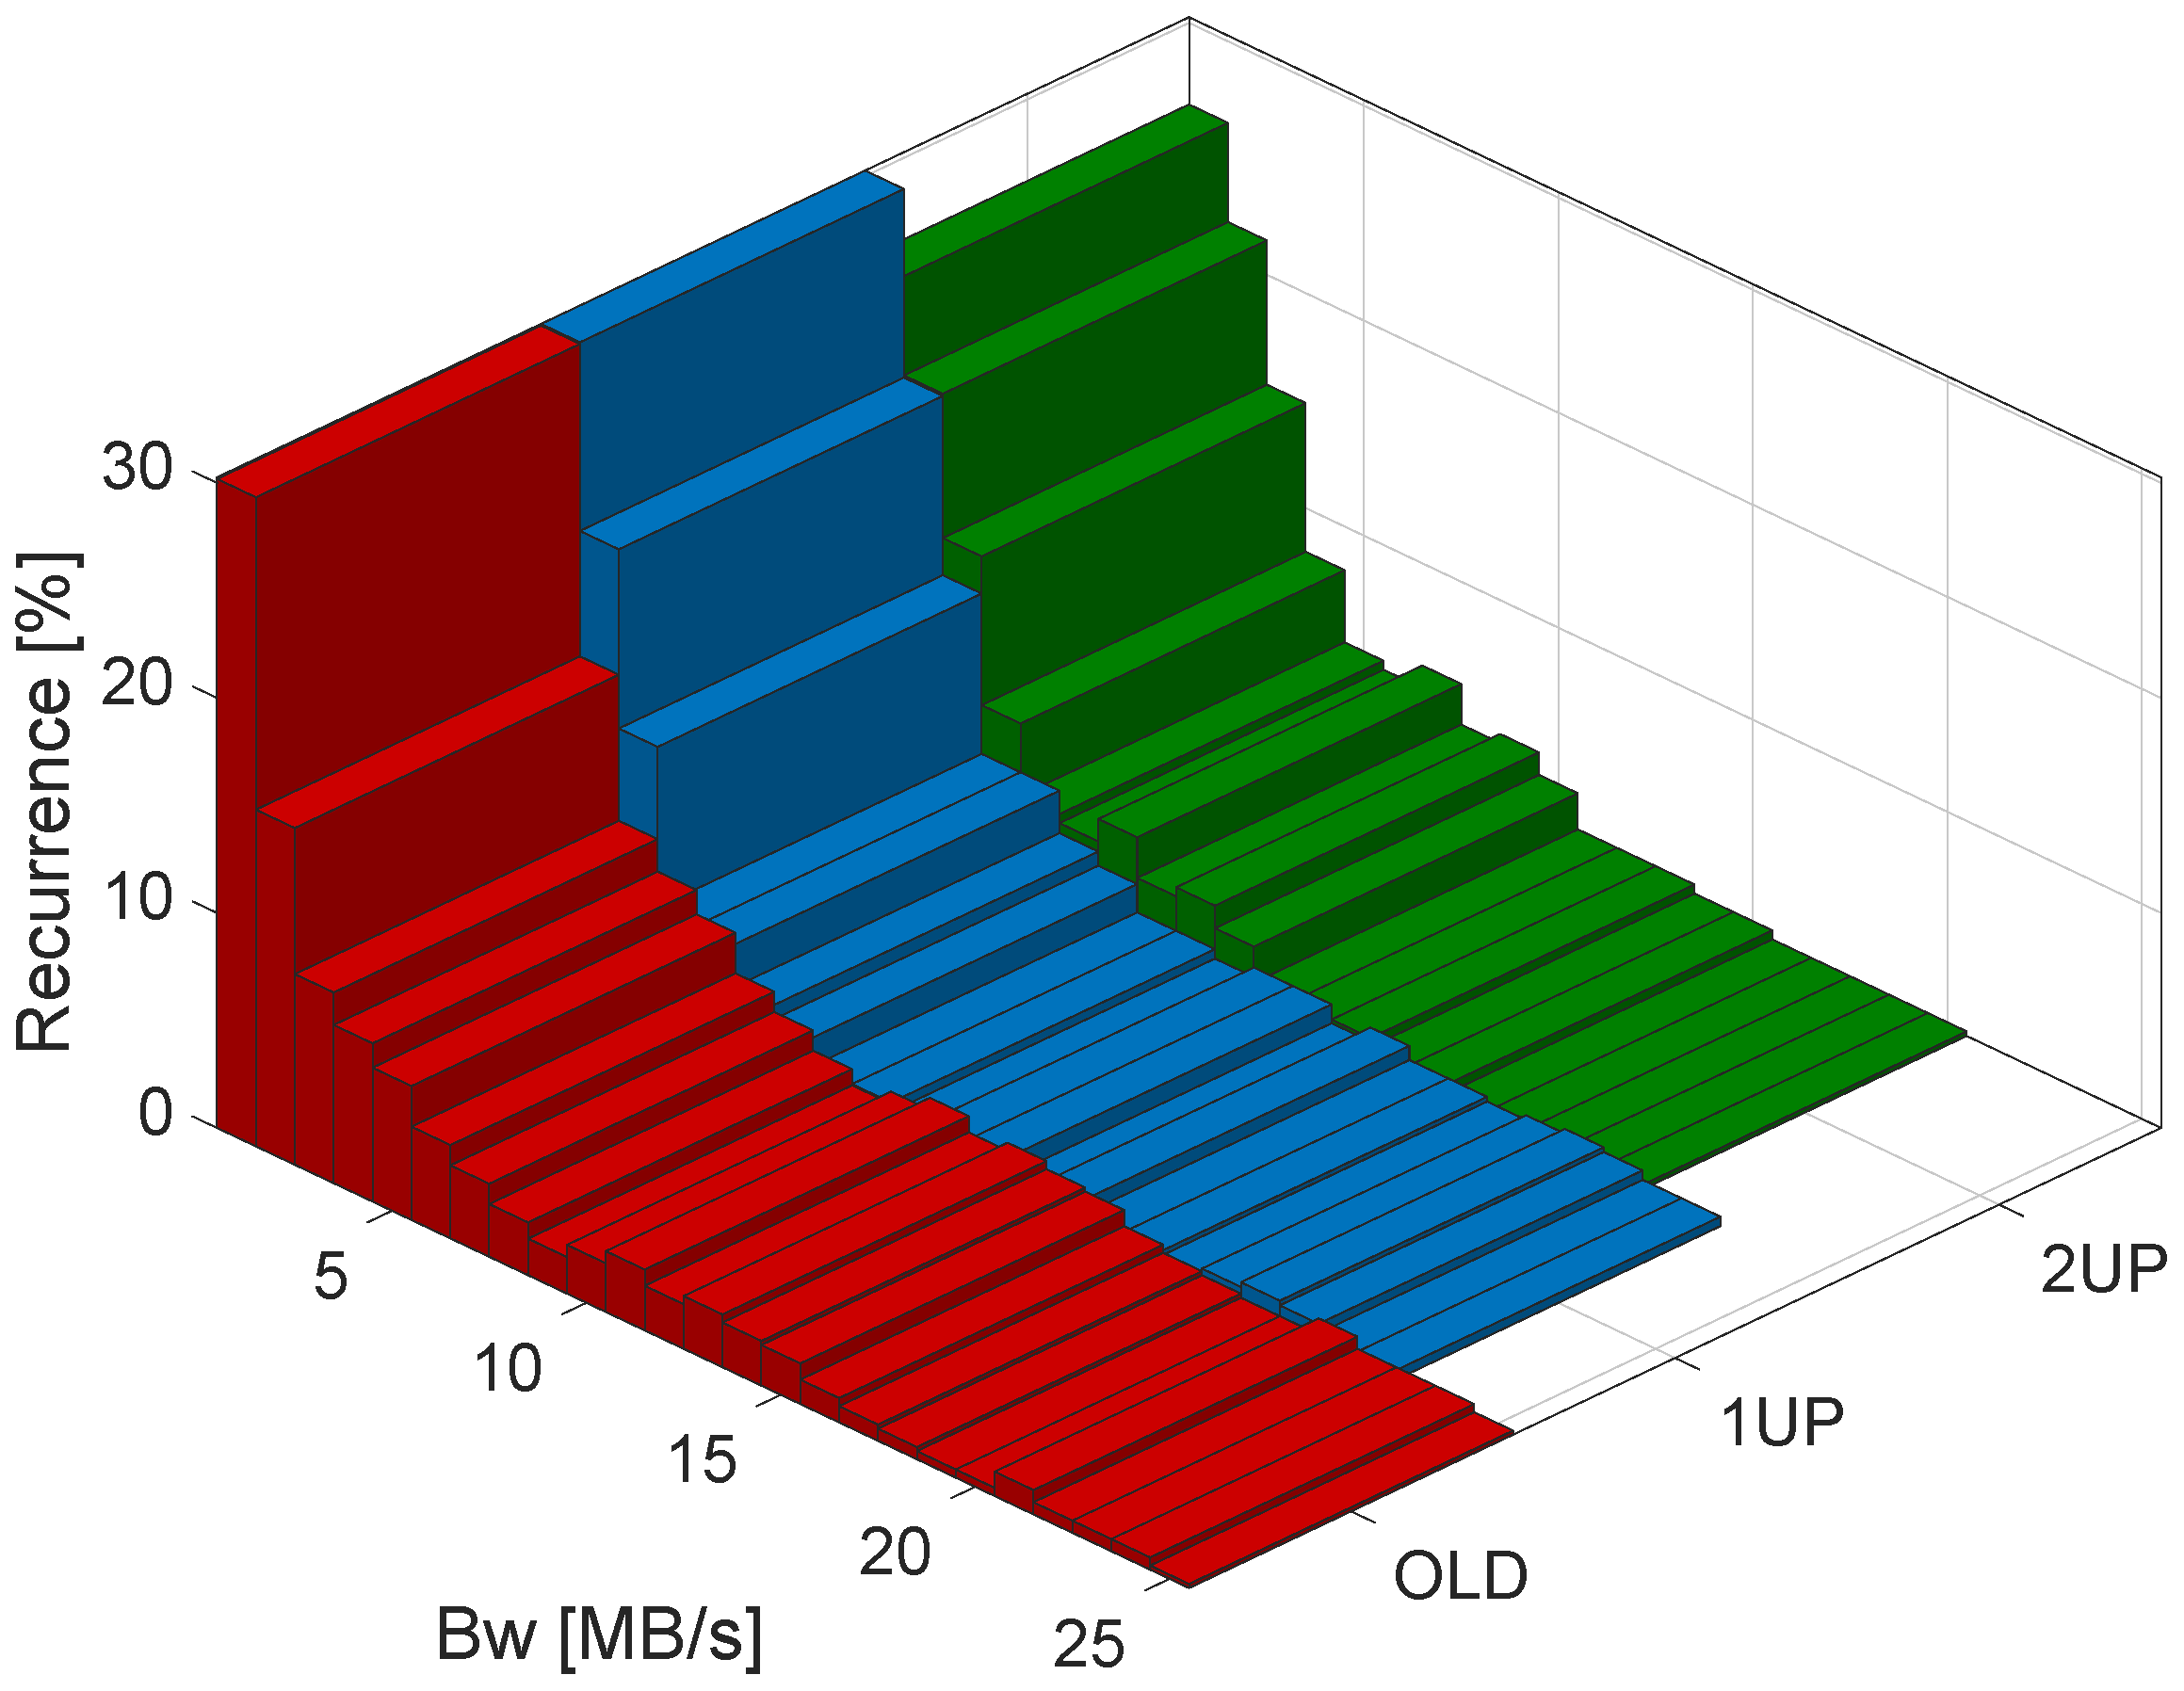
\includegraphics[width=0.7\linewidth]{figure/BW_NoPred.eps}}
\subfigure[b][]{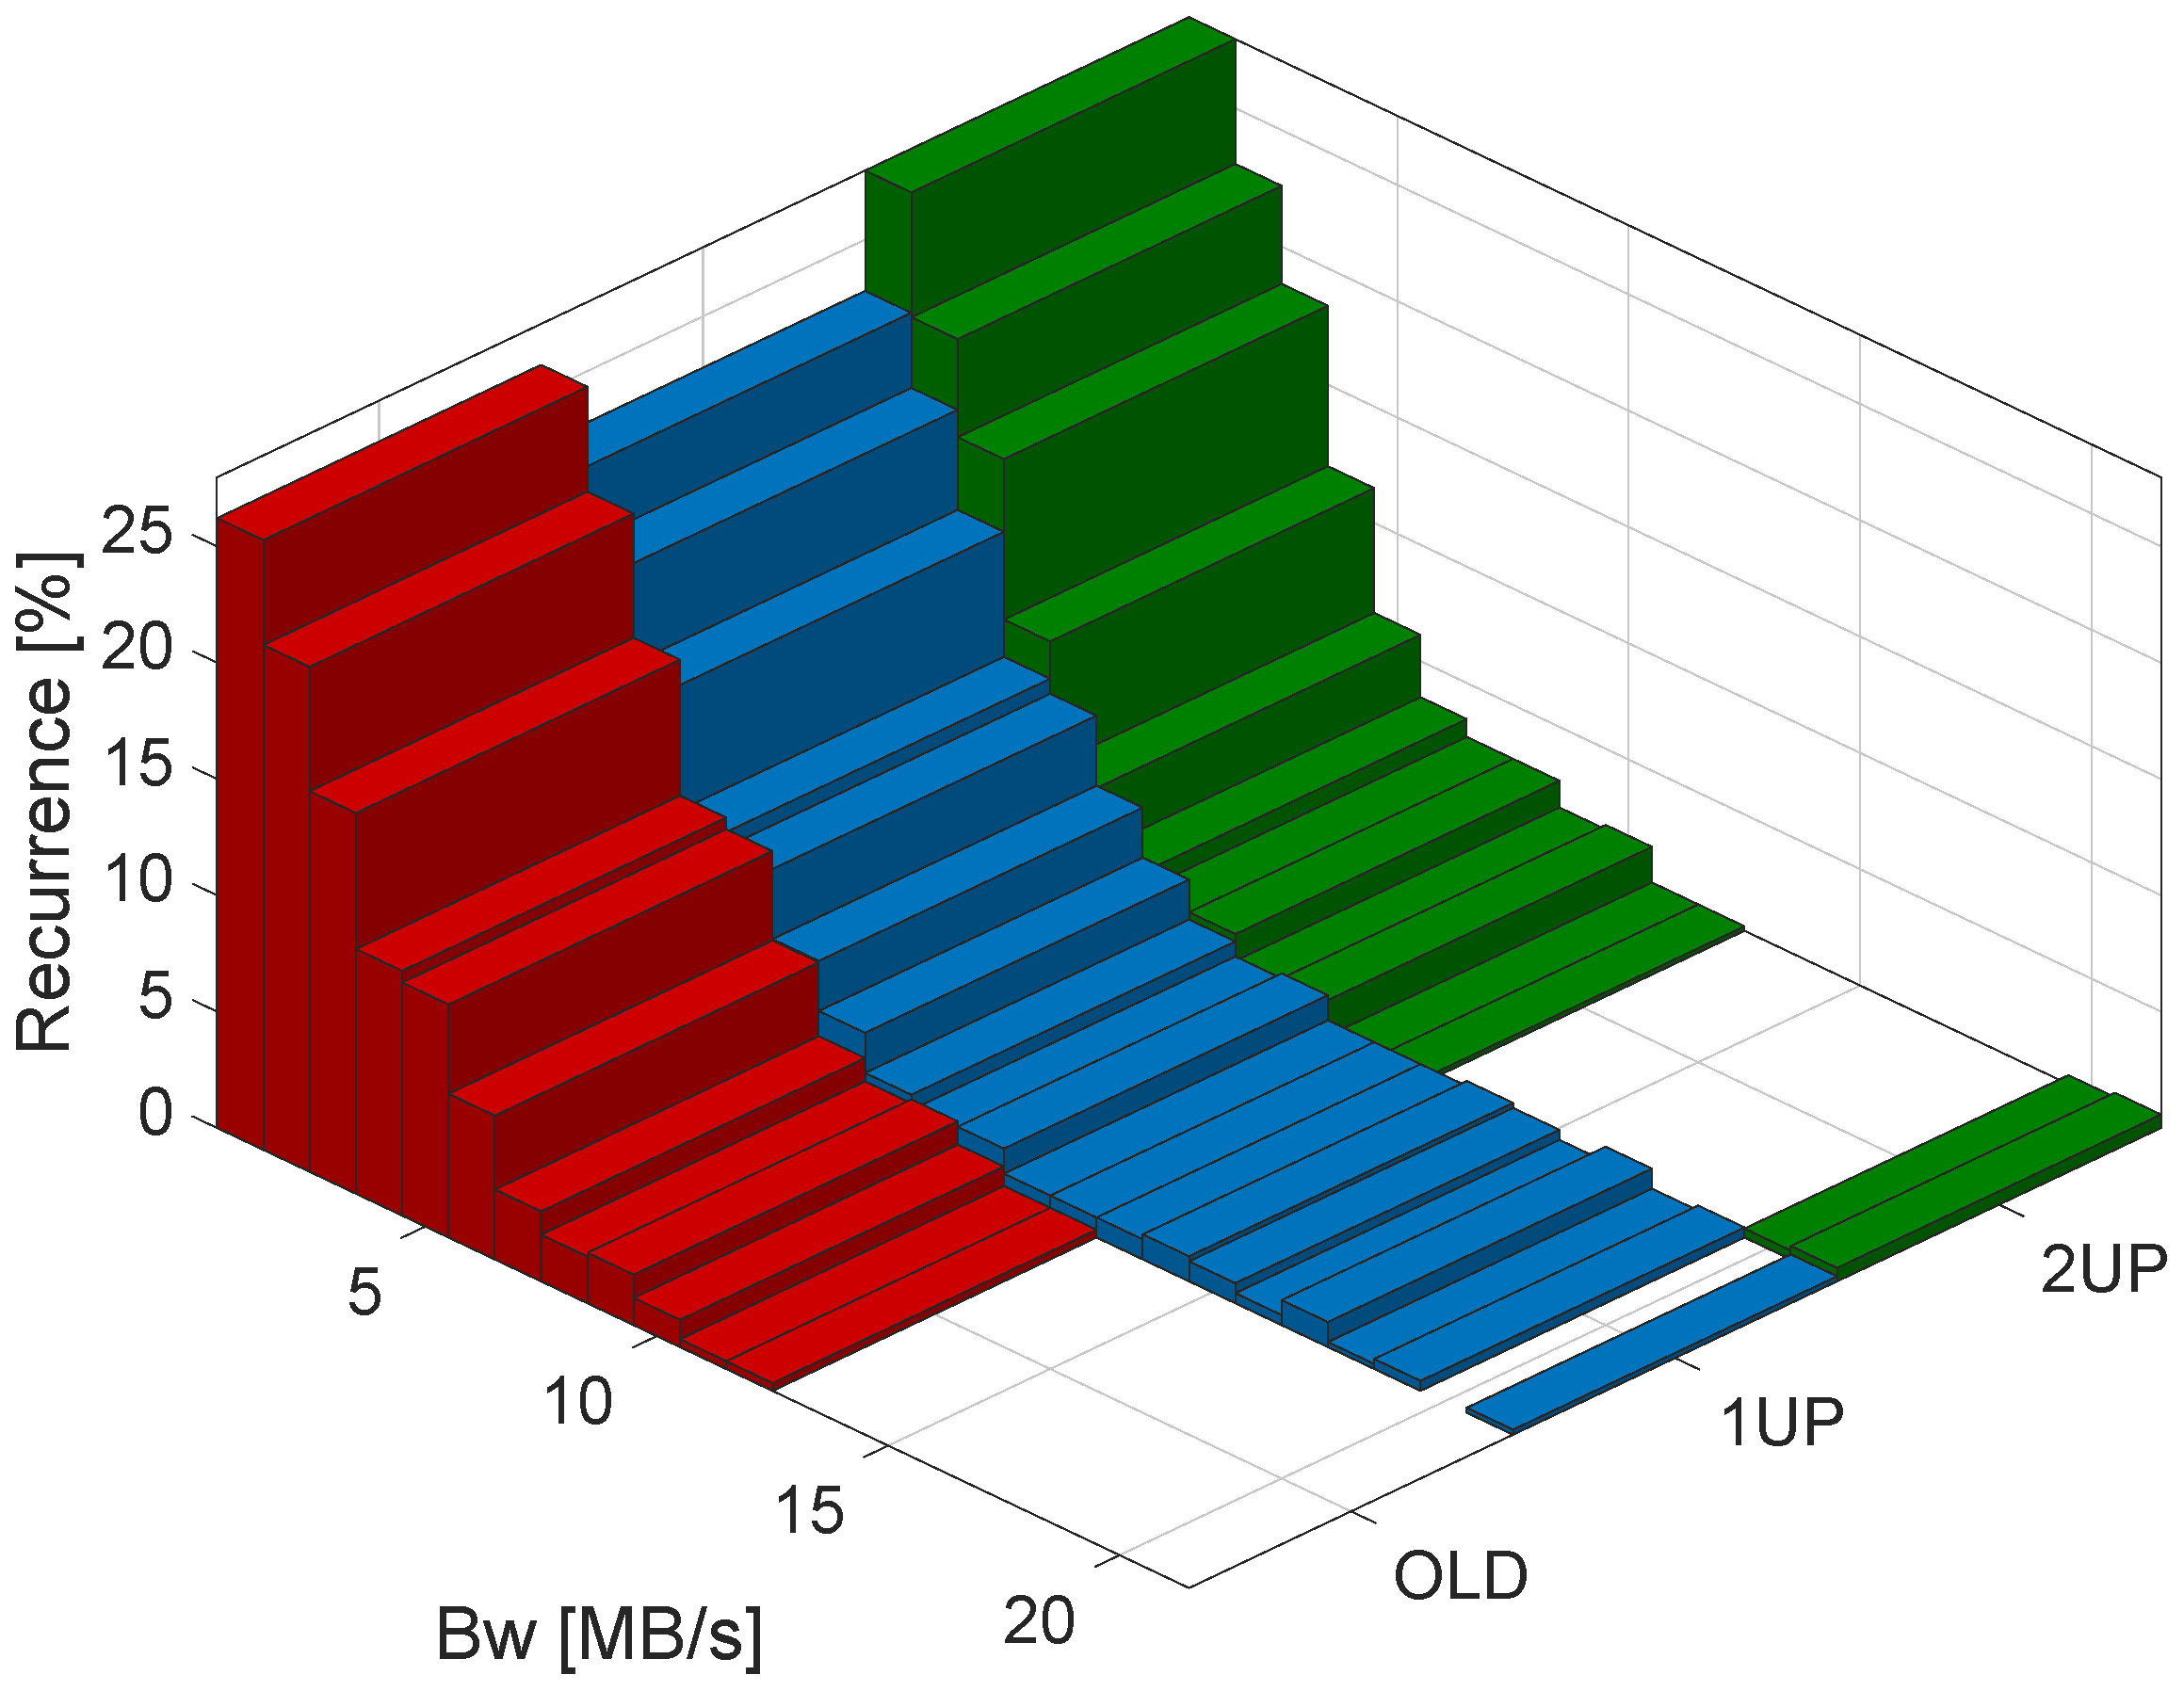
\includegraphics[width=0.7\linewidth]{figure/BW_Pred.eps}}
\caption{Bandwidth saving comparison without (a) and with (b) knowledge of the future disturbances.}
\label{fig:BW}
\end{figure}

Figure \ref{fig:BW} illustrates the bandwidth savings showing the recurrence of the different bandwidth usage during the simulations, respectively without and with knowledge of the future disturbances. Without disturbance forecast we exploited up to $25MB/s$ using the OLD model, while we exploited at most $22MB/s$ and $21MB/s$ respectively for models 1UP and 2UP. Using disturbance forecast, as expected, even less bandwidth is exploited.

\begin{figure}[h!]
\centering
\includegraphics[trim={120 0 120 0},width=0.9\linewidth]{figure/MPCfinal.eps}
\caption{Static controller up to the $400th$, then MPC controller.}
\label{fig:{MPC}}
\end{figure}
%\begin{figure}[h!]
%	\centering
%	\includegraphics[trim={120 0 120 0},width=0.7\linewidth]{figure/banda.eps}
%	\vspace{-0.2cm}
%	\caption{MPC controller: packets sent from the queues (orange), packets lost (red), bandwidth saving (blue).}
%	\vspace{-0.5cm}
%	\label{fig:{BWsave}}
%\end{figure}

We conclude this thesis by quantifying the gap between priority queueing control performance of MPC, obtained solving Problem \ref{pbMPC} and based on our RF predictive model, with the static control policy adopted by service provider networks in \cite{Notiziario}. Figure \ref{fig:{MPC}} highlights the dramatic improvement of MPC with respect to static control: the red line shows the incoming traffic, the blue line shows the sum of the packets sent from the queues, and their difference represents packet losses. Until the $400th$ static control has been implemented as in \cite{Notiziario}, generating many packet losses due to queues saturation. From that sample to the end of our experimentation we implemented MPC using our RF-based model, drastically reducing packet losses: quantitatively, after $700$ sampling periods the cumulative number of dropped packets with the static policy is about $5.5\cdot10^8$ versus $6.6\cdot10^6$ with MPC, with a decrease of $5.434\cdot10^8$ lost packets ($-88 \%$).
%Figure \ref{fig:{BWsave}} shows the amount of bandwidth that our method leaves unused at each time sample (blue line): during the simulation period we were able to save an average $3 MB/s$ with respect to static control, with peaks of more than $20 MB/s$, that can be of course allocated to improve the quality of other services.
We remark that, even thought the improvement of MPC with respect to static control is not surprising, much better performance can be obtained in real networks just collecting historical data and applying a controller that can be directly implemented using the accurate models of our identification algorithms and Quadratic Programming standard solvers.